
%% Preâmbulo (configurações, pacotes e tudo mais)
%% Preambulo LaTeX: Define classes e características do documento
%% Definição do docuemnto
\documentclass[
	%article,			% Define que este será um artigo (e não uma tese/monografia/relatório)
	12pt,				% Fonte: 12pt
	oneside,			% Impressão: oneside = 1 face, twoside = 2 faces (frente-e-verso)
    %openright,			% capítulos começam em página ímpar (use apenas se usar "twoside")
	a4paper,			% Tamanho do Papel: A4
    chapter=TITLE,		% Todos os capítulos devem ficam em caixa alta
    section=TITLE,		% Todas as seções devem ficar em caixa alta
	english,			% Adiciona Idioma para Hifenização: Inglês
    %spanish,			% Adiciona Idioma para Hifenização: Espanhol
    %french,			% Adiciona Idioma para Hifenização: Francês
	brazil				% Adiciona Idioma para Hifenização: Português do Brasil (o último idioma se torna o principal do documento)
]{abntex2}				% Utilizar ABNTeX2





%% Tipografia
%% Abra este arquivo e selecione uma das opções de fonte nele. A padrão é Times.
%% Tipografia / Fontes
%% AVISO: Todas essas fontes são *bastante semelhantes* aos nomes com as quais as descrevo. Entenda: são iguais, só que oficialmente com outro nome.

%% %%%%%%%%%%%%%%%%%%%%%%%%%%%%%%%%%%%%%%%%%%%%%%%%%%%%% %%
%% Comente todas as outras fontes que você não vai usar! %%
%% %%%%%%%%%%%%%%%%%%%%%%%%%%%%%%%%%%%%%%%%%%%%%%%%%%%%% %%

%% Latin Modern (fonte padrão do LaTeX, Computer Modern, mas com suporte a caracteres acentuados)
%% Considerada a mais clássica e bonita
%\usepackage{lmodern}



%% Times
%% Considerada a mais confortável de ler quando impresso
%%\usepackage{mathptmx}

%% Variação da mesma fonte, com minúsculas diferenças entre uma e outra (coisas bastante técnicas como kerning, aliasing e afins) - Essa tem revisões frequentes
%\usepackage{newtxtext} \usepackage{newtxmath}



%% Arial
%% Considerada mais confortável de ler num computador
%% ** Oficialmente recomendada pelo manual de formatação do IFPI **
\usepackage{helvet} \renewcommand{\familydefault}{\sfdefault}



%% Palatino
%% Uma opção mais elegante à Times
%\usepackage{newpxtext}



%% Kepler
%% Variação evoluída da Palatino, com várias pequenas diferenças e refinamentos
%\usepackage{kpfonts}



%% Libertine
%% Uma fonte estilo Serif comum no Linux
%\usepackage{libertine} %\usepackage[libertine]{newtxmath}



%% Pacotes usados pelo documento (se não entender não mexa, hehehe)
\usepackage{courier}                    % Permite a utilização da fonte Courier (para códigos-fonte)
\usepackage[T1]{fontenc}				% Seleção de códigos de fonte.
\usepackage[utf8]{inputenc}				% Codificação do documento (conversão automática dos acentos)
\usepackage{indentfirst}				% Indenta o primeiro parágrafo de cada seção.
\usepackage{nomencl} 					% Usado pela Lista de símbolos
\usepackage{color}						% Controle das cores
\usepackage{graphicx}					% Inclusão de gráficos
\usepackage{float}						% Melhorias para posicionamento de gráficos e tabelas
\usepackage{microtype} 					% Melhorias na justificação
\usepackage{lastpage}   		        % Dá acesso ao número da última página do documento
\usepackage{booktabs}					% Comandos para tabelas
\usepackage{multirow, array}			% Múltiplas linhas e colunas em tabelas
% \usepackage{titlesec}                   % Permite criar múltiplas sub seções
\usepackage[table,xcdraw]{xcolor}       % Cores para algumas tabelas especiais
% \usepackage[brazilian,hyperpageref]{backref}	 % Inclui nas Referências as páginas onde há as citações
\usepackage{simplecd}                   % Pacote para gerar capa do CD
\usepackage[final]{pdfpages}            % Pacote para incluir um PDF dentro de outro (ficha catalográfica)
\usepackage{csquotes}



%% Adiciona as alterações do ABNTeX-IFPI
\usepackage{abntex-ifpi/abntex-ifpi}

% Modificações do ABNTeX para o IFPI
\usepackage{abntex-ifpi/tikz-uml}	    % Pacote Tikz UML para criar UML no LaTeX





%% Metadados
%% Configurações dos metadados do PDF
\makeatletter
\hypersetup{
  pdftitle={\@title}, 
  pdfauthor={\@author},
  pdfsubject={\@title},
  pdfcreator={LaTeX, abntex2, {abnTeX\-ifpi}},
  %% Coloque aqui suas palavras-chave, cada uma entre chaves: {palavra}{palavra}{outra palavra}...
  pdfkeywords={palavra 1}{palavra 2}{palavra 3}{palavra 4}{palavra 5},
  colorlinks=true,			% Visual dos Links: false = caixas; true = colorido
  linkcolor=cor-link,		% Cor dos Links Internos (preto)
  citecolor=cor-link,		% Cor de Links para Bibliografia (preto)
  filecolor=cor-link,		% Cor para Links a Arquivos (preto)
  urlcolor=cor-link,		% Cor para Links a URLs (preto)
  bookmarksdepth=4
}
\makeatother



%% Metadados
%% %%%%%%%%%%%%%%%%%%%%%%%%%%%%%%%%%%%%%%%%%%%%%%%% %%
%% Metadados do trabalho
%% AVISO: Todos esses dados serão automaticamente convertidos para caixa alta onde necessário
%% %%%%%%%%%%%%%%%%%%%%%%%%%%%%%%%%%%%%%%%%%%%%%%%% %%

%% Título
\titulo{ViaBus: Plataforma para Gestão Integrada e Digitalização do Transporte Rodoviário Alternativo de Passageiros}

%% Autor
\autor{Jean Carlos Rodrigues Sousa}

%% Nome do Curso (usado para a Capa do CD)
\nomedocurso{Análise e Desenvolvimento de Sistemas}

%% Local de publicação
\local{Picos, Piauí}

%% Preâmbulo do trabalho
\preambulo{Trabalho de Conclusão de Curso (Relatório Técnico de Software) apresentado como exigência parcial para obtenção do diploma do Curso de Análise e Desenvolvimento de Sistemas do Instituto Federal de Educação, Ciência e Tecnologia do Piauí, Campus Picos.}

%% Orientador
%% "M\textsuperscript{e}." = Abreviação oficial para "Mestre"
\orientador{Prof. M\textsuperscript{e}. Jesiel Viana da Silva}

%% Tipo de Trabalho
%% - Monografia
%% - Tese (Mestrado)
%% - Tese (Doutorado)
%% - Relatório técnico
\tipotrabalho{Relatório Técnico de Software}

%% Data do Trabalho
\data{2025}

%% Nome da Instituição (para a capa)
\instituicao{INSTITUTO FEDERAL DE EDUCAÇÃO, CIÊNCIA E TECNOLOGIA DO PIAUÍ
\\
CAMPUS PICOS
\\
TECNOLOGIA EM ANÁLISE E DESENVOLVIMENTO DE SISTEMAS}

%% Primeiro membro da banca examinadora
\membroum{Prof. M\textsuperscript{e}. João Paulo Lima do Nascimento}

%% Segundo membro da banca examinadora
\membrodois{Prof. M\textsuperscript{e}. Jáder Anderson Oliveira de Abreu}

%% Terceiro membro da banca examinadora
%\membrotres{Prof. Dr. Xxxxxx Xxxxx}

%% Data da apresentação do trabalho
%% Se não souber a data da apresentação, utilize \underline{\hspace{3.5cm}}
%% Isso cria um sublinhado de 3.5cm, onde você pode escrever a data depois!
%\dataapresentacao{02 de Outubro de 2023}
\dataapresentacao{\underline{\hspace{1.0cm}}/\underline{\hspace{1.0cm}}/\underline{\hspace{1.75cm}}}



%% Configuração do "Citado nas páginas"
%% Configuração das Citações

%% Estilo
%\usepackage[num]{abntex2cite}			% Citações numéricas
% \usepackage[abnt-nbr10520=1988, alf, 
% abnt-emphasize = bf, 
% abnt-etal-list = 3,
% abnt-etal-text = it, 
% abnt-and-type = &, 
% abnt-last-names = abnt, 
% abnt-repeated-author-omit = no]{abntex2cite}			% Citações "AUTOR, ano"


% Definição do negrito

%% Colocar entre parênteses ou colchetes?
%% Padrão: Parênteses
%% * Fica mais agradável usar colchetes quando se usa citações numéricas
%\citebrackets[]							% Comente essa linha e o documento usará parênteses


%% Configura o "Citado nas Páginas ..." nas referências
%% Não mexa nesse:
% \renewcommand{\backref}{}

%% Esse é o texto do "Citado nas páginas ..."
% \renewcommand*{\backrefalt}[4]{
% 	\ifcase #1
% 		Nenhuma citação no texto.
% 	\or
% 		Citado na página #2.
% 	\else
% 		Citado #1 vezes nas páginas #2.
% 	\fi}

% ----------------------------------------------------------
% Referências e Citações no padrão da ABNT 2023
% ----------------------------------------------------------

\usepackage[style=abnt,
    backend=biber,
    maxbibnames=99,
    mincitenames=1,
    maxcitenames=3,
    backref=true,
    hyperref=true,
    giveninits=false,
    uniquename=false,
    uniquelist=false]{biblatex}

% Modificar a formatação do título do artigo para negrito
% \DeclareFieldFormat[article]{title}{\mkbibbold{#1}}

% Modificar a formatação do sobrenome em minúsculas
\renewcommand*{\mkbibnamefamily}[1]{#1}%

\addbibresource{bibliografia.bib}



%% Cores
%% Cores do Documento

%% Cor dos Links do PDF
%% Usando preta você "esconde" os links
\definecolor{cor-link}{RGB}{0,0,0}

%% Usando azul os links ficam visíveis (ruim para impressão)
%\definecolor{cor-link}{RGB}{8,40,75}



%% Cor para os quadros
%% Dê preferência a cores escuras.
%% Boa referência para cores: https://material.io/guidelines/style/color.html#color-color-palette
\definecolor{cor-quadro}{RGB}{5,28,63}		% Azul Escuro



%% Espaçamentos
%% Espaçamentos
%% O tamanho do parágrafo é dado por:
\setlength{\parindent}{1.5cm}

%% Espaçamento entre um parágrafo e outro:
%% O abntex diz: "tente também \onelineskip"
\setlength{\parskip}{0cm}


%% Início do Documento
\begin{document}

%% Documento será escrito em Português do Brasil
\selectlanguage{brazil}

%% Elementos pré-textuais: capa, folha de rosto, dedicatória, listas, sumário, etc.
%% %%%%%%%%%%%%%%%%%%%%%%%%%%%%%%%%%%%%%%%%% %%
%% Elementos Pré Textuais
%% ----------------------
%% 
%% Segundo o manual do IFPI, eles devem ser os seguintes (nessa ordem):
%%  1. Capa (obrigatório)
%%  2. Folha de rosto (obrigatório)
%%  3. Errata (opcional)
%%  4. Folha de aprovação (obrigatório)
%%  5. Dedicatória (opcional)
%%  6. Agradecimentos (opcional)
%%  7. Epígrafe (opcional)
%%  8. Resumo (obrigatório)
%%  9. Abstract/Resumo em outra língua (obrigatório)
%% 10. Lista de Ilustrações (opcional)
%% 11. Lista de Tabelas (opcional)
%% 12. Lista de Abreviaturas e Siglas (opcional)
%% 13. Lista de Símbolos (opcional)
%% 14. Sumário (obrigatório)
%% %%%%%%%%%%%%%%%%%%%%%%%%%%%%%%%%%%%%%%%%% %%

%% 01: Capa
\imprimircapa



%% 02: Folha de Rosto
%% OBS: O asterisco indica que haverá ficha bibliográfica (só funciona para impressão frente-e-verso)
\imprimirfolhaderosto*



%% Ficha Catalográfica (acho que é melhor adicionar via \includepdf depois)
%%% Ficha Catalográfica
%%
%% Este template cria um quadro semelhante a ficha catalográfica oficial.
%% É melhor usar \includepdf depois que a ficha oficial estiver em mãos.

%% Caso tenha o arquivo PDF da ficha
%% A ficha catalográfica do IFPI pode ser gerada através neste link: https://sistemas.ifpi.edu.br/fichacatalografica/
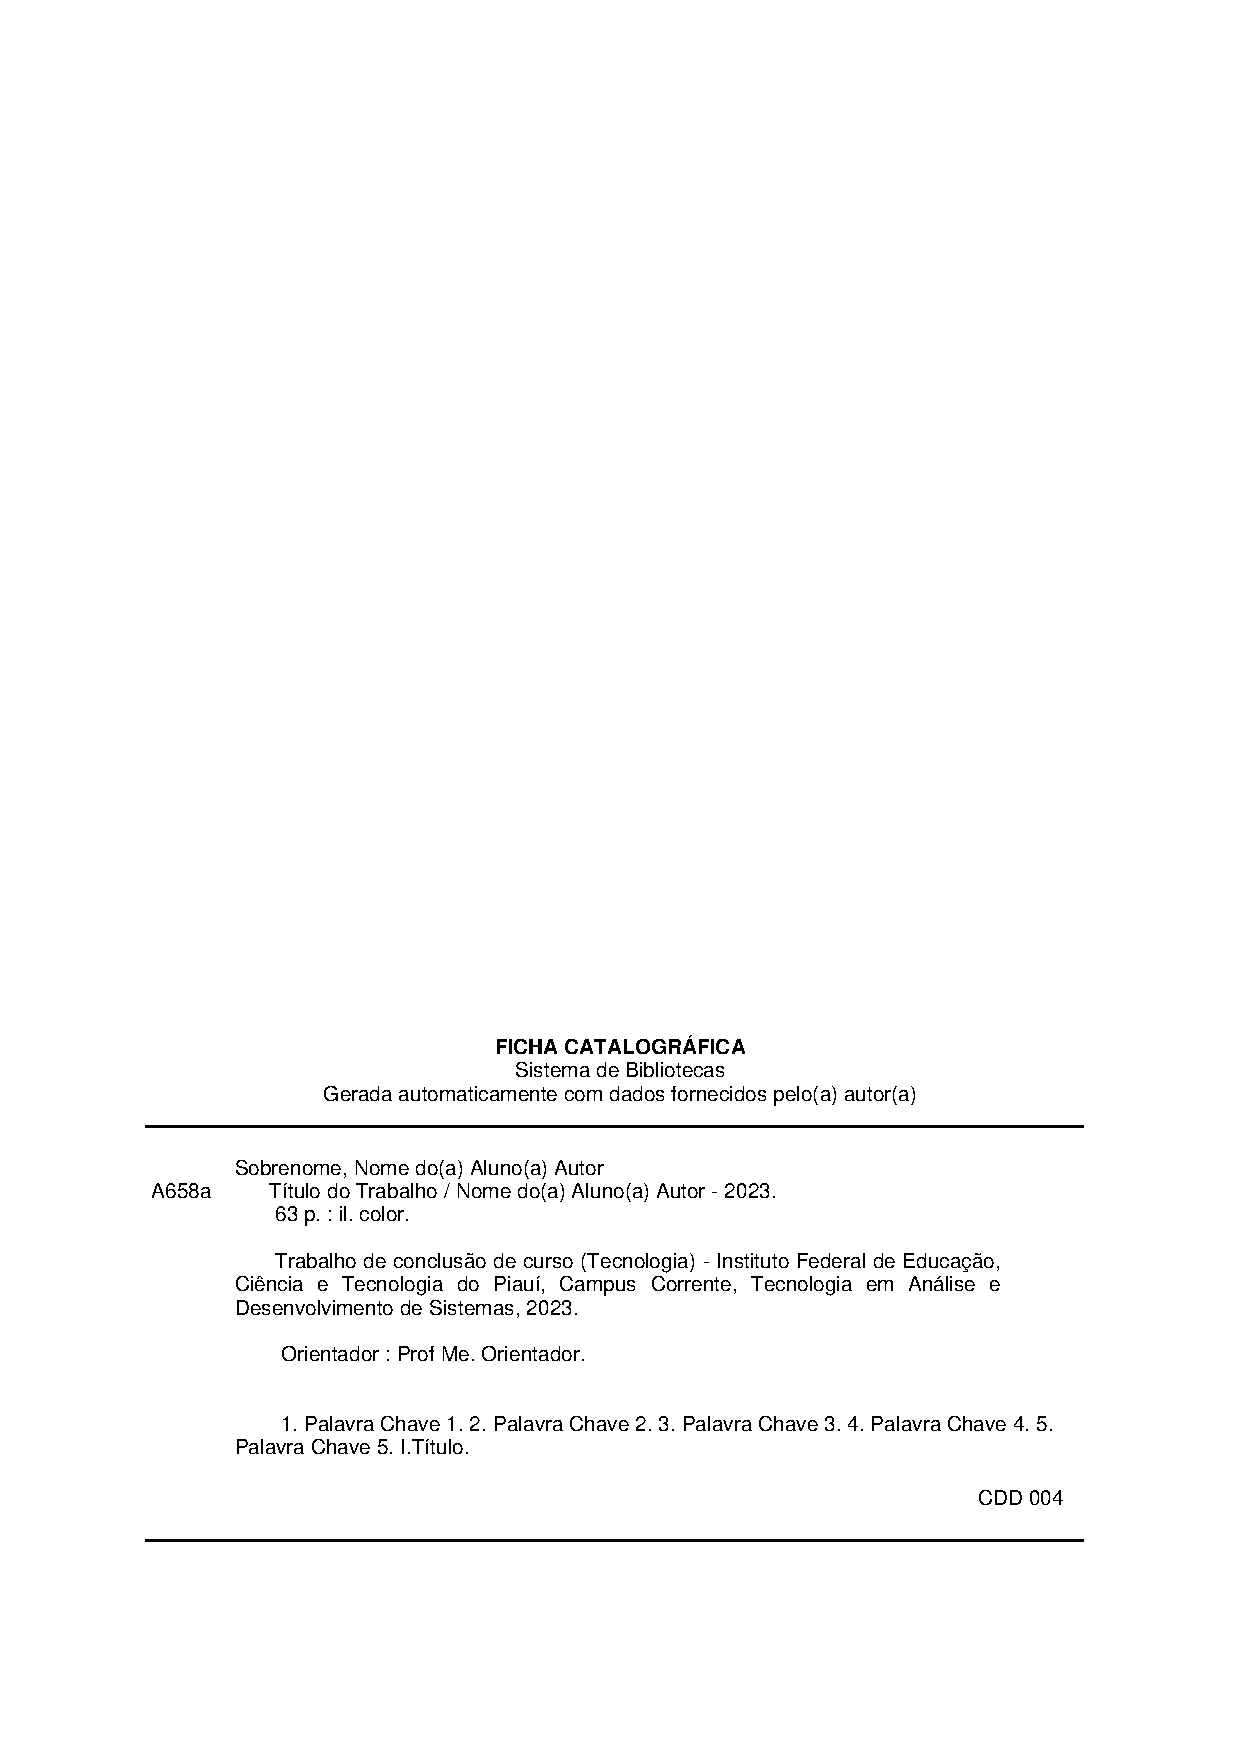
\includepdf{pre-textual/ficha-catalografica.pdf}

%% Caso queira fazer a ficha "tradicional" (este serve apenas como um modelo)
%\begin{fichacatalografica}
%	\sffamily
%	\vspace*{\fill}					% Posição vertical
%	\begin{center}					% Minipage Centralizado
%	\fbox{\begin{minipage}[c][8cm]{13.5cm}		% Largura
%	\small
%	\imprimirautor
%	
%	\hspace{0.5cm} \imprimirtitulo  / \imprimirautor. --
%	\imprimirlocal, \imprimirdata-
%	
%	\hspace{0.5cm} \thelastpage p. : il. (algumas color.) ; 30 cm.\\
%	
%	\hspace{0.5cm} \imprimirorientadorRotulo~\imprimirorientador\\
%	
%	\hspace{0.5cm}
%	\parbox[t]{\textwidth}{\imprimirtipotrabalho~--~\imprimirinstituicao,
%	\imprimirdata.}\\
%	
%	\hspace{0.5cm}
%		1. Palavra-chave1.
%		2. Palavra-chave2.
%		2. Palavra-chave3.
%		I. Orientador.
%		II. Universidade xxx.
%		III. Faculdade de xxx.
%		IV. Título 			
%	\end{minipage}}
%	\end{center}
%\end{fichacatalografica}


%% 03: Errata
%% Errata
%\begin{errata}
%Elemento opcional da norma ABNT NBR14724 de 2011. Exemplo:
%
%\vspace{\onelineskip}
%
%FERRIGNO, C. R. A. \textbf{Tratamento de neoplasias ósseas apendiculares com reimplantação de enxerto ósseo autólogo autoclavado associado ao plasma rico em plaquetas}: estudo crítico na cirurgia de preservação de membro em cães. 2011. 128 f. Tese (Livre-Docência) - Faculdade de Medicina Veterinária e Zootecnia, Universidade de São Paulo, São Paulo, 2011.

%% Tabela de exemplo com os erros
%\begin{table}[htb]
%\center
%\footnotesize
%\begin{tabular}{|p{1.4cm}|p{1cm}|p{3cm}|p{3cm}|}
%  \hline
%   \textbf{Folha} & \textbf{Linha}  & \textbf{Onde se lê}  & \textbf{Leia-se}  \\
%    \hline
%    1 & 10 & auto-conclavo & autoconclavo\\
%   \hline
%\end{tabular}
%\end{table}
%
%\end{errata}



%% 04: Folha de Aprovação
\imprimirfolhadeaprovacao
%% Use esta se forem 4 membros na banca:
%\imprimirfolhadeaprovacaoduascolunas



%% 05: Dedicatória
%% Dedicatória do seu trabalho
\begin{dedicatoria}
	%% Empura o texto a seguir para a parte de baixo da página
	\vspace*{\fill}
    
    %% Alinhado a Direita
    \center
    \begin{flushright}
    	Dedico este trabalho à minha família, cujo apoio e incentivo tornaram possível esta nova jornada.
    \end{flushright}
    
    %% Descomente a linha seguir para deixar o texto centralizado verticalmente na página
    %% Lembre de comentar o "\begin{}" e "\end{}" acima para centralizar o texto da dedicatória.
	%\vspace*{\fill}
\end{dedicatoria}



%% 06: Agradecimentos
%% Agradecimentos
\begin{agradecimentos}
  Agradeço primeiramente a Deus, por me conceder força e perseverança ao longo desta caminhada.
  
  Ao meu orientador, Prof. Me. Aislan Rafael Rodrigues de Sousa, pelo apoio, paciência e orientação fundamentais para a realização deste trabalho.
  
  Aos meus pais, Josué José Filho e Maria de Fátima Rodrigues, por todo o apoio, suporte e incentivo ao longo da minha jornada acadêmica.
  
  Aos professores do curso de Análise e Desenvolvimento de Sistemas do IFPI – Campus Picos, por compartilharem conhecimento e contribuírem para minha formação profissional.
  
  E, com imensa gratidão, à minha parceira Karielly de Carvalho, por estar ao meu lado, apoiando-me em todos os momentos.
  
  A todos que, de alguma forma, fizeram parte desta jornada, meu sincero agradecimento.
  \end{agradecimentos}



%% 07: Epígrafe
%% Epígrafe
%% Uma frase que lhe inspira ou a qual lhe inspirou a fazer este trabalho
\begin{epigrafe}
  \vspace*{\fill}
  \begin{flushright}
  \emph{"Software é uma grande combinação de arte e engenharia.”. 
    \\ Bill Gates}
  \end{flushright}
  \end{epigrafe}



%% 08: Resumo
%% Resumo
\begin{resumo}
  O setor de transporte rodoviário alternativo de passageiros carece de soluções tecnológicas acessíveis, resultando em uma gestão predominantemente manual, fragmentada e ineficiente. Este trabalho aborda este problema através do projeto e desenvolvimento de um protótipo funcional de uma plataforma web, denominada ViaBus, no modelo Software as a Service (SaaS). A metodologia adotada partiu de uma pesquisa de mercado qualitativa para o levantamento de requisitos, seguida pela modelagem de uma arquitetura de software multi-tenant e a implementação do protótipo com as tecnologias NestJS para o backend e Next.js para o frontend. Como resultado, foi entregue uma aplicação funcional que centraliza o gerenciamento de frotas, motoristas, rotas e a venda de passagens, com a verificação de requisitos confirmando a implementação do núcleo operacional. Adicionalmente, uma avaliação heurística da interface indicou uma base de usabilidade sólida, com forte aderência a princípios de consistência e clareza, embora tenha apontado oportunidades de melhoria na prevenção de erros. Conclui-se que a abordagem SaaS com foco na simplicidade é uma solução tecnicamente viável para o nicho de mercado estudado, e que o protótipo ViaBus serve como uma prova de conceito eficaz dessa proposta, com suas limitações e oportunidades de trabalhos futuros devidamente documentadas.
  \vspace{\onelineskip}
  \noindent
  
  \textbf{Palavras-chave}: Transporte de Passageiros; Software como Serviço; Sistema de Gestão; Arquitetura de Software.
  \end{resumo}

%% 09: Abstract/Resumo em língua estrangeira
%% Abstract (configurado para língua inglesa)
\begin{resumo}[Abstract]    % Título do Resumo (Abstract = Resumo em inglês)
  \begin{otherlanguage*}{english}  % Língua do texto
  The alternative road passenger transport sector lacks accessible technological solutions, resulting in predominantly manual, fragmented, and inefficient management. This work addresses this problem through the design and development of a functional prototype of a web platform, named ViaBus, based on the Software as a Service (SaaS) model. The adopted methodology started with a qualitative market research for requirements gathering, followed by the modeling of a multi-tenant software architecture and the implementation of the prototype using NestJS for the backend and Next.js for the frontend. As a result, a functional application was delivered that centralizes the management of fleets, drivers, routes, and ticket sales, with the requirements verification confirming the implementation of the operational core. Additionally, a heuristic evaluation of the interface indicated a solid usability foundation, with strong adherence to principles of consistency and clarity, although it pointed out opportunities for improvement in error prevention. It is concluded that the SaaS approach focused on simplicity is a technically feasible solution for the studied market niche, and that the ViaBus prototype serves as an effective proof of concept for this proposal, with its limitations and opportunities for future work duly documented.
  
  \vspace{\onelineskip}
  \noindent
  \textbf{Keywords}: Passenger Transportation; Software as a Service; Management System; Software Architecture.
  \end{otherlanguage*}
  \end{resumo}



%% 10: Lista de Ilustrações
%% Lista de Ilustrações
\pdfbookmark[0]{\listfigurename}{lof}
\listoffigures*
\cleardoublepage



%% 11: Lista de Tabelas
%% Lista de Tabelas
%\pdfbookmark[0]{\listtablename}{lot}
%\listoftables*
%\cleardoublepage



%% 12: Lista de Abreviaturas e Siglas
%% Lista de Siglas
\begin{siglas}
  \item[ABNT] Associação Brasileira de Normas Técnicas
  \item[CRB] Conselho Regional de Biblioteconomia
  \item[IBGE] Instituto Brasileiro de Geografia e Estatística
  \item[IFPI] Instituto Federal de Educação, Ciência e Tecnologia do Piauí
  \item[UFPI] Universidade Federal do Piauí
\end{siglas}



%% 13: Lista de Símbolos
%% Lista de Símbolos
%% (esta é apenas uma lista de exemplo)
\begin{simbolos}
  \item [\% ] Porcentagem
  \item [ © ] Copyright
  \item [ ® ] Marca registrada
  \item [ \$ ] Dólar
  \item [ § ] Seção
  \item[$ \Gamma $] Letra grega Gama
  \item[$ \Lambda $] Lambda
  \item[$ \zeta $] Letra grega minúscula zeta
  \item[$ \in $] Pertence
\end{simbolos}



%% 14: Sumário (o asterisco retira o próprio sumário do sumário)
\pdfbookmark[0]{\contentsname}{toc}
\tableofcontents*
\cleardoublepage



%% Indica que a partir daqui ficarão os elementos textuais (TCC em si)
\textual

%% Inclui os capítulos do TCC (parte textual)
%% %%%%%%%%%%%%%%%%%%%%%%%%%%%%%%%%%%% %%
%% Elementos Textuais (Capítulos)      %%
%% %%%%%%%%%%%%%%%%%%%%%%%%%%%%%%%%%%% %%
\pagestyle{empty} % Remover cabeçalho com titulo dos capítulos


%% Inclua aqui os capítulos que farão parte do TCC
\chapter{Introdução}\label{cha:introducao}

Em um país de dimensões continentais, o transporte rodoviário de passageiros funciona como um elemento estratégico para a integração socioeconômica, conectando municípios e garantindo a mobilidade da população \cite{FGV2023}. Enquanto o sistema interestadual é regulamentado em nível federal pela Agência Nacional de Transportes Terrestres (ANTT), conforme estabelecido em sua lei de criação \cite{BRASIL2001}, uma vasta e heterogênea rede de transporte intermunicipal opera sob jurisdição estadual.

No estado do Piauí, esta modalidade é uma realidade consolidada, cuja organização é definida pela Lei Nº 8.562 de 2025, que dispõe sobre o Sistema de Transporte Rodoviário Intermunicipal de Passageiros do Estado do Piauí (STRIP/PI). A referida lei classifica o "serviço alternativo"\ como uma das categorias oficiais do sistema, designando a Secretaria dos Transportes (SETRANS) como o poder concedente \cite{PIAUI2025}. Este serviço, prestado por veículos de menor porte, surge para suprir as lacunas deixadas pelo sistema convencional. A existência de uma legislação específica demonstra a relevância do setor, mas também evidencia a necessidade de ferramentas de gestão que se adaptem às suas particularidades operacionais.

Diante desse cenário, este trabalho propõe o desenvolvimento de uma plataforma
baseada no modelo Software como Serviço (\textit{SaaS, Software as a Service})
para a gestão integrada de empresas de transporte rodoviário alternativo.
A escolha por este modelo se fundamenta na definição de Chong e Carraro
(2006 apud \textcite{melo2007software}) como um "software implementado
como um serviço hospedado e acessado pela Internet", o que permite que empresas
utilizem soluções baseadas em nuvem com custos operacionais reduzidos e alta
escalabilidade --- características especialmente vantajosas para o setor em foco.

Este cenário, onde um serviço regulamentado e essencial como o transporte alternativo ainda opera com uma gestão predominantemente analógica — fato constatado na pesquisa de mercado realizada para este trabalho (\autoref{apendice:resultados}) —, evidencia os desafios para a modernização do setor. A ausência de sistemas de gestão integrados e a consequente dependência de processos manuais não apenas comprometem a eficiência operacional e a qualidade dos serviços prestados, mas também criam uma barreira para a inovação e o crescimento sustentável das empresas que atuam nesse segmento.

\section{Justificativa}

O transporte rodoviário alternativo de passageiros no Brasil, embora essencial para a conectividade regional, opera de forma majoritariamente analógica e fragmentada. Uma pesquisa de mercado realizada para este estudo (\autoref{apendice:resultados}) revelou que a gestão de frotas e a venda de passagens ainda são fortemente dependentes de processos manuais, como o uso de cadernos de anotações e planilhas. Essa carência de ferramentas digitais integradas limita a eficiência e o potencial de crescimento do setor. Neste contexto, a adoção de plataformas \textit{SaaS} surge como uma solução estratégica para transformar esse cenário, otimizando recursos e reduzindo custos operacionais. Estudos de mercado mais amplos corroboram essa visão, indicando que tecnologias no setor de transportes podem elevar a eficiência logística em até 15\% \cite{setcepar2023}.

Além disso, uma plataforma \textit{SaaS} voltada para o transporte alternativo pode facilitar o acesso à inovação para pequenas e médias empresas, sem exigir altos investimentos. Esse modelo permite automação da bilhetagem, gestão integrada de rotas e melhor experiência para o passageiro. Essas soluções já demonstram impacto positivo em outros segmentos do transporte, aumentando a competitividade e garantindo serviços mais confiáveis \cite{prologapp2024}. Assim, a digitalização do setor não só fortalece as empresas, mas também melhora a mobilidade interurbana, tornando os serviços mais eficientes e acessíveis.

\section{Objetivos}

\subsection{Geral}

Desenvolver um protótipo funcional de uma plataforma SaaS para a gestão integrada do transporte rodoviário alternativo de passageiros, verificando a implementação de suas funcionalidades essenciais e avaliando a usabilidade de sua interface a partir de princípios de design.

\subsection{Específicos}

\begin{itemize}
    \item Realizar uma pesquisa de mercado para identificar as dores e os processos manuais de empresas do setor de transporte alternativo;

    \item Especificar os requisitos funcionais e não funcionais de um sistema de gestão com base nas necessidades levantadas na pesquisa;

    \item Desenvolver um protótipo funcional da plataforma ViaBus, implementando os módulos de gestão de rotas, paradas, veículos, motoristas e um fluxo para agendamento de passagens;

    \item Realizar uma verificação técnica do protótipo para analisar a aderência do software aos requisitos especificados e conduzir uma avaliação heurística para identificar possíveis melhorias de usabilidade na interface.
\end{itemize}

\section{Metodologia}

A metodologia empregada para a concepção e desenvolvimento do sistema ViaBus foi estruturada em três etapas sequenciais: levantamento de requisitos, desenvolvimento do protótipo e avaliação da solução.

A primeira etapa, de levantamento de requisitos, utilizou uma abordagem mista, partindo da observação empírica do autor sobre os desafios do setor de transporte alternativo. Tais observações foram então validadas por meio de uma pesquisa de mercado qualitativa. Para tal, foi elaborado um questionário online (detalhado no \autoref{apendice:questionario}) e aplicado junto a gestores de duas empresas do setor. As respostas, consolidadas na tabela do \autoref{apendice:resultados}, foram essenciais para a especificação formal dos requisitos que nortearam o desenvolvimento.

A segunda etapa, de desenvolvimento do protótipo, seguiu um processo iterativo alinhado a práticas de prototipagem evolutiva, onde o software é construído e refinado em ciclos contínuos \cite{sommerville2011software}. Adotou-se a estratégia \textit{Frontend-First}, que prioriza a construção da interface do usuário (UI) como guia para o desenvolvimento do sistema. Utilizando o framework Next.js e a biblioteca de componentes shadcn/ui, todas as telas da aplicação foram inicialmente desenvolvidas com dados estáticos (\textit{mockados}), permitindo a validação dos fluxos de interação antes da implementação da lógica de negócio no backend.

Por fim, a terceira etapa consistiu na avaliação do protótipo. Devido à impossibilidade de realizar testes com usuários finais, optou-se por uma verificação interna em duas frentes. A primeira foi uma \textit{Verificação de Requisitos}, na qual se analisou sistematicamente o atendimento aos requisitos funcionais e não funcionais. A segunda foi uma \textit{Avaliação Heurística}, um método de inspeção consolidado para encontrar problemas de usabilidade em interfaces \cite{Nielsen1994}. Atuando como avaliador especialista, o autor inspecionou o sistema com base nas 10 heurísticas de usabilidade de Nielsen, cujos resultados detalhados são apresentados no Capítulo 5.
% % ----------------------------------------------------------
% % Fundamentação Teórica
% % ----------------------------------------------------------
% \chapter{Fundamentação Teórica}
% \label{cha:fundamentacao_teorica}

% Neste capítulo, são apresentados os conceitos essenciais que fundamentam o desenvolvimento deste trabalho. A primeira seção aborda o modelo \textit{Software as a Service} (SaaS), detalhando sua definição, arquitetura, vantagens e desafios. A segunda seção explora a aplicação de tecnologias no setor de transporte rodoviário, destacando como as plataformas SaaS podem otimizar a gestão e a eficiência operacional.

% \section{Software as a Service (SaaS)}

% O modelo \textit{Software as a Service} (SaaS), ou Software como Serviço, representa uma mudança de paradigma na forma como o software é distribuído e consumido. Em vez de adquirir licenças de uso perpétuo e instalar o software em servidores locais, os usuários acessam a aplicação pela internet, geralmente por meio de um navegador web, pagando uma taxa recorrente (assinatura) pelo serviço \cite{salesforce2025saas}.

% Nesse modelo, toda a infraestrutura subjacente — servidores, armazenamento, redes e o próprio software — é gerenciada pelo provedor do serviço. Isso significa que o fornecedor é responsável pela manutenção, atualizações, segurança e disponibilidade da aplicação, permitindo que as empresas clientes foquem em suas atividades principais sem se preocupar com a complexidade da gestão de TI \cite{microsoft2025azure}.

% \subsection{Arquitetura e Modelo de Negócio}

% A arquitetura mais comum em soluções SaaS é a \textit{multi-tenancy} (multilocação), onde uma única instância da aplicação e da infraestrutura serve a múltiplos clientes (locatários ou \textit{tenants}). Embora compartilhem os mesmos recursos computacionais, os dados de cada cliente são mantidos isolados e seguros, garantindo a privacidade e a confidencialidade das informações \cite{microsoft2025learn}. Essa abordagem permite que o provedor otimize os recursos e reduza os custos, o que se reflete em preços mais acessíveis para o cliente final.

% O modelo de negócio é baseado em assinaturas, que podem variar em preço conforme o número de usuários, os recursos contratados ou o volume de uso. Essa flexibilidade oferece escalabilidade, permitindo que as empresas ajustem o serviço de acordo com seu crescimento e suas necessidades, pagando apenas pelo que utilizam \cite{prologapp2024}.

% \subsection{Vantagens e Desafios}

% A adoção de plataformas SaaS oferece um conjunto significativo de vantagens para as empresas, especialmente para as de pequeno e médio porte, que podem não dispor de grandes orçamentos para investimentos em tecnologia. Entre os principais benefícios, destacam-se:

% \begin{itemize}
%     \item \textbf{Redução de Custos:} Elimina a necessidade de altos investimentos iniciais em hardware e licenças de software. Os custos de manutenção, atualização e suporte técnico também são responsabilidade do provedor \cite{prologapp2024}.
%     \item \textbf{Acessibilidade e Mobilidade:} Por ser acessado via internet, o software pode ser utilizado de qualquer lugar e em diferentes dispositivos, bastando uma conexão ativa.
%     \item \textbf{Escalabilidade:} As empresas podem facilmente aumentar ou diminuir a quantidade de recursos e usuários conforme a demanda, sem a necessidade de reestruturar a infraestrutura de TI.
%     \item \textbf{Atualizações Automáticas:} O provedor é responsável por manter o software atualizado com as últimas funcionalidades e correções de segurança, garantindo que todos os clientes utilizem sempre a versão mais recente da aplicação \cite{gestran2025saas}.
%     \item \textbf{Implementação Rápida:} A configuração e o início do uso de um sistema SaaS são geralmente mais rápidos em comparação com a instalação de um software tradicional (on-premise).
% \end{itemize}

% Apesar das vantagens, o modelo também apresenta desafios que devem ser considerados. A principal desvantagem é a dependência de uma conexão estável com a internet para acessar o serviço. Além disso, as opções de personalização podem ser mais limitadas em comparação com soluções desenvolvidas internamente, e a segurança dos dados, embora robusta, fica sob a responsabilidade de um terceiro, o que exige uma análise cuidadosa na escolha do fornecedor \cite{agendor2025b2b}.

% \section{Tecnologia no Setor de Transporte Rodoviário}

% O setor de transporte rodoviário de passageiros, historicamente caracterizado por processos manuais e uma gestão descentralizada, tem passado por uma profunda transformação impulsionada pela tecnologia. A digitalização das operações não apenas otimiza a gestão, mas também melhora a experiência do cliente e a segurança nas estradas.

% Ferramentas como Sistemas de Gerenciamento de Transporte (TMS, \textit{Transportation Management System}), roteirizadores inteligentes e plataformas de venda online de passagens tornaram-se cruciais para a competitividade das empresas. Um TMS, por exemplo, centraliza informações sobre frotas, motoristas, rotas e finanças, permitindo um controle mais eficaz e uma tomada de decisão baseada em dados \cite{praxio2023tecnologia}.

% \subsection{O Papel das Plataformas SaaS no Transporte}

% As plataformas SaaS surgem como uma solução ideal para democratizar o acesso a essas tecnologias avançadas no setor de transporte alternativo. Ao oferecer um sistema robusto em um modelo de serviço, as barreiras de custo e complexidade técnica são drasticamente reduzidas.

% Uma plataforma SaaS voltada para o transporte rodoviário, como a proposta neste trabalho, pode integrar diversas funcionalidades essenciais em um único ambiente. Segundo a Point Sistemas (2025), a aplicação desse modelo na logística permite obter visibilidade total da operação em tempo real, incluindo o acompanhamento de veículos, a gestão de ocorrências e a otimização de rotas com base em dados como geolocalização e tempo estimado de viagem \cite{pointsistemas2025logistica}.

% A automação de tarefas, como a emissão de bilhetes, o controle de embarque e o fechamento financeiro, reduz a incidência de erros manuais e libera a equipe para se concentrar em atividades estratégicas. Além disso, a capacidade de integrar-se facilmente com outras ferramentas, como sistemas financeiros e de CRM, cria um ecossistema tecnológico coeso e eficiente, fundamental para a modernização e o crescimento sustentável do setor \cite{gestran2025saas}.


% ----------------------------------------------------------
% Fundamentação Teórica
% ----------------------------------------------------------

\chapter{Fundamentação Teórica}
\label{cha:fundamentacao_teorica}

Neste capítulo, são apresentados os conceitos essenciais que fundamentam o desenvolvimento deste trabalho. A primeira seção aborda o modelo \textit{Software as a Service} (SaaS), detalhando sua definição, arquitetura, vantagens e desafios. A segunda seção explora a aplicação de tecnologias no setor de transporte rodoviário, e a terceira aprofunda-se na arquitetura e nas tecnologias específicas escolhidas para a construção do protótipo.

\section{Software as a Service (SaaS)}

O modelo \textit{Software as a Service} (SaaS), ou Software como Serviço, representa uma mudança de paradigma na forma como o software é distribuído e consumido. Diferentemente do modelo tradicional \textit{on-premise}, onde o cliente adquire licenças e é responsável pela infraestrutura, no modelo SaaS o cliente paga uma assinatura periódica para acessar a aplicação pela internet, que é hospedada na nuvem pelo provedor do serviço \cite{moveideias2025saas}.

Nesse modelo, toda a infraestrutura subjacente — servidores, armazenamento, redes e o próprio software — é gerenciada pelo provedor. Isso significa que o fornecedor é responsável pela manutenção, atualizações, segurança e disponibilidade da aplicação, permitindo que as empresas clientes foquem em suas atividades principais sem se preocupar com a complexidade da gestão de TI \cite{moveideias2025saas}.

\subsection{Arquitetura e Modelo de Negócio}

A arquitetura mais comum em soluções SaaS é a \textit{multi-tenancy} (multilocação), onde uma única instância da aplicação e da infraestrutura serve a múltiplos clientes (locatários ou \textit{tenants}) \cite{frontegg2021multitenant}. Embora compartilhem os mesmos recursos computacionais, os dados de cada cliente são mantidos isolados e seguros, garantindo a privacidade e a confidencialidade das informações. Essa abordagem permite que o provedor otimize os recursos e reduza os custos, o que se reflete em preços mais acessíveis para o cliente final.

O modelo de negócio é baseado em assinaturas, que podem variar em preço conforme o número de usuários, os recursos contratados ou o volume de uso. Essa flexibilidade oferece escalabilidade, permitindo que as empresas ajustem o serviço de acordo com seu crescimento e suas necessidades, pagando apenas pelo que utilizam \cite{prologapp2024saas}.

\subsection{Vantagens e Desafios para PMEs}

A adoção de plataformas SaaS oferece um conjunto significativo de vantagens estratégicas para as Pequenas e Médias Empresas (PMEs). A principal delas é a drástica \textbf{redução de custos}, pois o modelo de assinatura elimina a necessidade de altos investimentos de capital (CAPEX) em licenças e hardware, transformando-os em despesas operacionais (OPEX) previsíveis \cite{praxio2021vantagens}.

Outros benefícios incluem \cite{prologapp2024saas, praxio2021vantagens}:
\begin{itemize}
    \item \textbf{Escalabilidade e Flexibilidade:} As empresas podem facilmente aumentar ou diminuir a capacidade de uso do software para responder rapidamente às mudanças do mercado.
    \item \textbf{Acessibilidade e Mobilidade:} Por ser acessado via internet, o software pode ser utilizado de qualquer lugar e em diferentes dispositivos, algo transformador para o setor de logística, permitindo que gestores monitorem operações remotamente e equipes externas capturem dados em tempo real.
    \item \textbf{Foco no \textit{Core Business}:} Ao terceirizar a gestão da infraestrutura de TI, as PMEs podem dedicar mais tempo e recursos para a otimização das operações logísticas e atendimento ao cliente.
    \item \textbf{Segurança e Disponibilidade:} Provedores de SaaS geralmente oferecem um nível de segurança e redundância de infraestrutura superior ao que uma PME poderia implementar por conta própria, garantido por Acordos de Nível de Serviço (SLAs).
\end{itemize}

Apesar das vantagens, o modelo também apresenta desafios, como a dependência de uma conexão estável com a internet e opções de personalização potencialmente mais limitadas.

\section{Tecnologia e Inovação no Transporte Rodoviário}

O setor de transporte rodoviário de passageiros, apesar de sua importância socioeconômica, apresenta um ritmo lento na adoção de tecnologias digitais \cite{sestsenat2021relatorio}. A ausência de soluções tecnológicas integradas, especialmente no segmento alternativo, resulta em ineficiências como a falta de controle sobre os processos, a incapacidade de atender a picos de demanda e altos índices de reclamação de clientes \cite{fateczl2022impactos}.

Plataformas SaaS surgem como uma solução ideal para democratizar o acesso a tecnologias avançadas neste setor. A análise de soluções comerciais existentes, como TOTVS, iTransport e Praxio, revela uma lacuna de mercado: as ferramentas ou são muito complexas e caras para PMEs, ou são focadas em nichos específicos como o fretamento corporativo, não atendendo de forma integrada as necessidades do operador de transporte alternativo \cite{totvs2025passageiros, itransport2025gestao, praxioluna2025venda}.

\section{Arquitetura Tecnológica da Solução Proposta}

A concepção de uma plataforma robusta, escalável e de fácil manutenção depende das escolhas arquitetônicas e tecnológicas. Cada componente da arquitetura foi selecionado estrategicamente para maximizar a produtividade, garantir a qualidade do software e mitigar riscos de desenvolvimento.

\subsection{Tecnologias do Backend}

O backend é o alicerce da plataforma, responsável pela lógica de negócios, persistência de dados e segurança. A \textit{stack} escolhida foi projetada para ser modular, robusta e escalável, utilizando tecnologias consolidadas no ecossistema TypeScript.

\subsubsection{NestJS e Arquitetura Modular}
O framework escolhido para o desenvolvimento do backend foi o NestJS. Trata-se de um framework Node.js progressivo, construído com e para o TypeScript, que utiliza uma arquitetura fortemente modular \cite{nestjs2025framework}. O pilar do NestJS é o conceito de Módulos, que organizam o código em blocos coesos e funcionais (e.g., um módulo para autenticação, outro para gestão de rotas). Cada módulo encapsula seus próprios \textit{controllers}, \textit{providers} (serviços) e pode importar ou exportar funcionalidades \cite{nestjs2025modules}. Essa estrutura promove uma forte separação de responsabilidades, facilita a reutilização de código e a manutenção do sistema, sendo ideal para a plataforma proposta, onde funcionalidades complexas podem ser desenvolvidas como módulos independentes \cite{devanddeliver2024architecture}.

\subsubsection{TypeORM e Mapeamento Objeto-Relacional (ORM)}
Para a camada de persistência de dados, a escolha foi o TypeORM. Um \textit{Object-Relational Mapper} (ORM) é uma técnica que cria uma ponte entre o paradigma orientado a objetos da aplicação e o paradigma relacional dos bancos de dados, permitindo que os desenvolvedores manipulem o banco de dados através de objetos e classes, abstraindo a necessidade de escrever consultas SQL manualmente \cite{logrocket2024typeorm}. O TypeORM é um ORM maduro para o ecossistema TypeScript, que utiliza intensivamente decoradores para definir Entidades (classes que mapeiam para tabelas) de forma declarativa e fortemente tipada. Isso acelera o desenvolvimento e reduz a probabilidade de erros relacionados a dados \cite{devto2024typeorm}.

\subsubsection{Autenticação com JWT e Passport.js}
A segurança da API é um requisito crítico. A estratégia de autenticação escolhida foi baseada em \textit{JSON Web Tokens} (JWT), implementada com a biblioteca Passport.js. JWT é um padrão aberto (RFC 7519) para a criação de tokens de acesso compactos e autossuficientes. Quando um cliente faz uma requisição a um recurso protegido, ele envia o JWT, e o servidor pode verificar a assinatura para autenticar o usuário sem precisar consultar um banco de dados de sessões, resultando em uma autenticação \textit{stateless} ideal para APIs RESTful \cite{soshace2024jwt}. O Passport.js atua como um \textit{middleware} de autenticação modular, e a estratégia \textit{passport-jwt} é projetada especificamente para extrair e verificar a validade desses tokens, oferecendo uma solução robusta e padronizada para proteger as rotas da API \cite{passportjs2025jwt}.

\subsection{Tecnologias do Frontend}

A interface do usuário (\textit{frontend}) é o principal ponto de contato com os gestores e passageiros. Sua arquitetura foi projetada com foco em performance e robustez, utilizando um ecossistema moderno baseado em React.

\subsubsection{Next.js, SSR e App Router}
O framework escolhido para o frontend é o Next.js. Uma de suas principais características é o suporte nativo à Renderização no Servidor (\textit{Server-Side Rendering} - SSR), na qual a página HTML é gerada no servidor a cada requisição. Isso melhora o tempo de carregamento inicial da página e a otimização para motores de busca (SEO) \cite{medium2025ssr}. Com a introdução do \textit{App Router}, o Next.js adotou por padrão o uso de \textit{React Server Components}, que permitem que a busca de dados e a renderização de componentes não interativos ocorram exclusivamente no servidor. Isso resulta em uma redução significativa da quantidade de JavaScript enviada ao cliente e otimiza a performance geral da aplicação \cite{nextjs2025servercomponents}.

\subsubsection{React, TypeScript e Ecossistema de UI}
A base da interface é o React, uma biblioteca JavaScript para a construção de interfaces baseada em um modelo de componentes reutilizáveis. Para garantir a robustez e a manutenibilidade, o React é utilizado com o TypeScript, um superconjunto do JavaScript que adiciona tipagem estática. O TypeScript permite a detecção de erros em tempo de compilação e serve como uma forma de documentação viva, tornando o código mais fácil de entender e facilitando a colaboração \cite{dhiwise2024reacttypescript}.

Para a estilização, foi adotado o Tailwind CSS, um framework \textit{utility-first} que acelera o desenvolvimento e garante consistência visual \cite{medium2025cssframeworks}. Comple-mentando-o, a biblioteca de componentes \textit{shadcn/ui} foi utilizada. Diferente de bibliotecas tradicionais, seus componentes são copiados para o código-fonte do projeto, dando ao desenvolvedor controle total sobre o código e permitindo personalizações profundas sem \textit{vendor lock-in} \cite{shadcnui2025docs}.

\subsubsection{Gerenciamento de Formulários e Validação}
Para a gestão de formulários e a validação de dados, foi utilizada a combinação do React Hook Form com a biblioteca Zod. O React Hook Form se destaca pela sua performance, minimizando re-renderizações desnecessárias \cite{reacthookform2025getstarted}. O Zod é uma biblioteca de validação de esquemas \textit{TypeScript-first} que permite definir regras de validação de forma declarativa e, a partir delas, inferir automaticamente os tipos TypeScript correspondentes. A integração entre as duas cria um sistema de validação de formulários poderoso e com segurança de tipos de ponta a ponta \cite{contentful2024zod}.

\subsection{Conteinerização com Docker}

Para garantir a consistência do ambiente de desenvolvimento e simplificar o processo de implantação, a aplicação e seus serviços dependentes (como o banco de dados) foram conteinerizados usando Docker. O Docker é uma plataforma que permite empacotar uma aplicação e todas as suas dependências em uma unidade padronizada e isolada chamada contêiner. Isso garante que a aplicação funcione da mesma forma em qualquer ambiente, seja na máquina de um desenvolvedor ou em produção, eliminando o clássico problema de "funciona na minha máquina" \cite{docker2025overview}. Através de arquivos de configuração como o \texttt{Dockerfile} (que descreve como construir a imagem da aplicação) e o \texttt{docker-compose.yml} (que orquestra múltiplos contêineres), o processo de setup e implantação é simplificado e padronizado.

% ----------------------------------------------------------
% Tecnologias Envolvidas
% ----------------------------------------------------------
\chapter{Arquitetura e Modelagem do Sistema} \label{cha:arquitetura}

\section{Arquitetura da Solução}
Esta seção descreve a organização estrutural do sistema BusLy, que provê funções de gestão de transporte para empresas: cadastro de empresas, usuários, motoristas, veículos, rotas, paradas, viagens e bilhetes. A solução adota uma arquitetura web em camadas, com separação clara entre apresentação (frontend), lógica de negócio e APIs (backend) e persistência (banco de dados).

No \textit{frontend}, utiliza-se Next.js~15 com roteamento via App Router, estado de sessão via NextAuth (estratégia \textit{JWT}) e componentes React tipados (TypeScript). O \textit{frontend} consome APIs REST autenticadas, mantém contexto de usuário/empresa e incorpora mapas e edição geográfica com Leaflet/React-Leaflet para operações sobre rotas e paradas.

O \textit{backend} é implementado com NestJS~11, estruturado por módulos de domínio (\textit{auth}, \textit{users}, \textit{companies}, \textit{drivers}, \textit{vehicles}, \textit{stops}, \textit{routes}, \textit{trips}, \textit{tickets}, etc.). As regras de negócio são expostas por controladores REST, protegidos por autenticação \textit{JWT} e autorização baseada em papéis. A multiempresa é tratada por \textit{companyId} e por um interceptor que injeta o contexto de empresa a partir do token. A persistência usa TypeORM com PostgreSQL.

\begin{figure}[H]
\centering
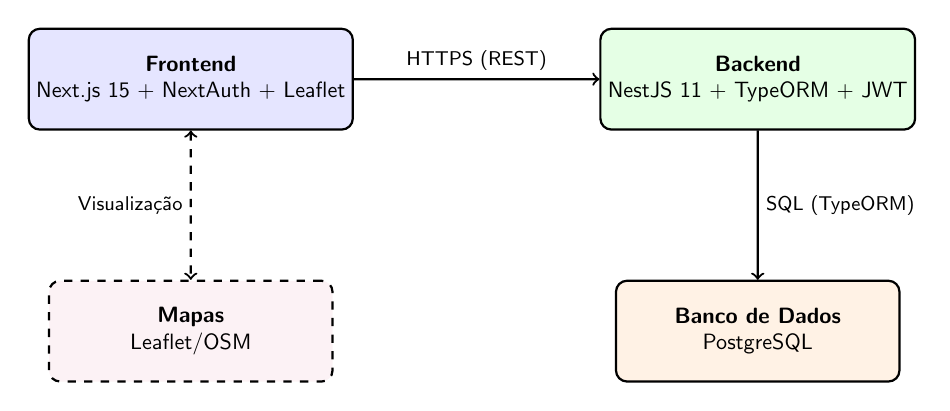
\begin{tikzpicture}[scale=0.8, every node/.style={transform shape}]
  \tikzumlset{font=\footnotesize}
  % Blocos
  \node[draw, rounded corners, thick, fill=blue!10, minimum width=4.5cm, minimum height=1.6cm, align=center] (fe) at (0,2) {\textbf{Frontend}\\Next.js 15 + NextAuth + Leaflet};
  \node[draw, rounded corners, thick, fill=green!10, minimum width=4.5cm, minimum height=1.6cm, align=center] (be) at (9,2) {\textbf{Backend}\\NestJS 11 + TypeORM + JWT};
  \node[draw, rounded corners, thick, fill=orange!10, minimum width=4.5cm, minimum height=1.6cm, align=center] (db) at (9,-2) {\textbf{Banco de Dados}\\PostgreSQL};
  \node[draw, dashed, rounded corners, thick, fill=purple!5, minimum width=4.5cm, minimum height=1.6cm, align=center] (maps) at (0,-2) {\textbf{Mapas}\\Leaflet/OSM};

  % Conexões
  \draw[->, thick] (fe) -- node[above, font=\small]{HTTPS (REST)} (be);
  \draw[->, thick] (be) -- node[right, font=\small]{SQL (TypeORM)} (db);
  \draw[<->, thick, dashed] (fe) -- node[left, font=\small]{Visualização} (maps);
\end{tikzpicture}
\caption{Visão de alto nível da solução.}
\end{figure}

\section{Modelagem do Banco de Dados}
O modelo de dados foi projetado para refletir as agregações de negócio. A Tabela~\ref{tab:principais-entidades} sumariza as principais entidades e seus papéis. De forma geral, todas as entidades operacionais são associadas a uma empresa (\textit{multi-tenancy} por chave estrangeira \texttt{company\_id}). Rotas possuem paradas ordenadas (\texttt{route\_stops}) e agenda de operação (\texttt{route\_schedules}); viagens instanciam rotas em horários específicos e originam bilhetes.

\begin{table}[H]
\centering
\begin{tabular}{ll}
\toprule
\textbf{Entidade} & \textbf{Descrição resumida} \\
\midrule
\texttt{companies} & Empresa (razão social, nome fantasia, CNPJ, slug, contato) \\
\texttt{users} & Usuário (nome, e-mail, senha, papel, status, \texttt{company\_id}) \\
\texttt{drivers} & Motorista (CPF, CNH, categoria, status, \texttt{company\_id}) \\
\texttt{vehicles} & Veículo (placa, capacidade, categoria, status, \texttt{company\_id}) \\
\texttt{addresses} & Endereço (CEP, logradouro, geocoordenadas) \\
\texttt{stops} & Parada (nome, \texttt{address\_id}, acessibilidade, \texttt{company\_id}) \\
\texttt{routes} & Rota (nome, distância, duração estimada, \texttt{company\_id}) \\
\texttt{route\_stops} & Associação rota–parada com ordem e horário opcional \\
\texttt{route\_schedules} & Agenda por dia da semana para a rota \\
\texttt{trips} & Viagem (rota, janelas horárias, status, assentos, \texttt{company\_id}) \\
\texttt{tickets} & Bilhete (passageiro, preço, assento, pontos de embarque) \\
\bottomrule
\end{tabular}
\caption{Principais entidades do domínio.}
\label{tab:principais-entidades}
\end{table}

O diagrama de classes da Figura~\ref{fig:uml-dominio} sintetiza os relacionamentos mais relevantes do domínio.

\begin{figure}[H]
\centering
\begin{tikzpicture}[scale=0.4, every node/.style={transform shape}]
  \tikzumlset{font=\tiny}
  
  % NÍVEL 1: Empresa (topo da hierarquia)
  \umlclass[x=18,y=25]{Company}{
    id: uuid\\
    legalName: string\\
    tradeName: string\\
    slug: string\\
    cnpj: string\\
    email: string\\
    phone: string\\
    logoUrl: string\\
    createdAt: Date\\
    updatedAt: Date
  }{ }
  
  % NÍVEL 2: Gestão de usuários e recursos
  \umlclass[x=3,y=18]{User}{
    id: uuid\\
    name: string\\
    email: string\\
    phone: string\\
    photoUrl: string\\
    password: string\\
    role: UserRole\\
    status: UserStatus\\
    companyId: uuid\\
    createdAt: Date\\
    updatedAt: Date
  }{ }
  
  \umlclass[x=18,y=18]{Vehicle}{
    id: uuid\\
    plate: string\\
    model: string\\
    brand: string\\
    year: number\\
    capacity: number\\
    category: VehicleCategory\\
    comfortConfiguration: ComfortConfiguration\\
    busType: BusType\\
    acquisitionDate: Date\\
    odometer: number\\
    lastMaintenance: Date\\
    nextMaintenance: Date\\
    status: VehicleStatus\\
    notes: string\\
    companyId: uuid
  }{ }
  
  \umlclass[x=33,y=18]{Driver}{
    id: uuid\\
    name: string\\
    cpf: string\\
    licenseNumber: string\\
    licenseCategory: string\\
    licenseExpiry: Date\\
    phone: string\\
    email: string\\
    birthDate: Date\\
    hireDate: Date\\
    status: DriverStatus\\
    emergencyContactName: string\\
    emergencyContactPhone: string\\
    address: string\\
    notes: string\\
    companyId: uuid
  }{ }
  
  % NÍVEL 3: Configuração de rotas
  \umlclass[x=8,y=11]{Route}{
    id: uuid\\
    name: string\\
    description: string\\
    isActive: boolean\\
    estimatedDuration: string\\
    distance: number\\
    companyId: uuid
  }{ }
  
  \umlclass[x=23,y=11]{Stop}{
    id: uuid\\
    name: string\\
    addressId: uuid\\
    isActive: boolean\\
    hasAccessibility: boolean\\
    hasShelter: boolean\\
    companyId: uuid
  }{ }
  
  \umlclass[x=38,y=11]{Address}{
    id: uuid\\
    cep: string\\
    street: string\\
    number: string\\
    complement: string\\
    neighborhood: string\\
    city: string\\
    state: string\\
    longitude: number\\
    latitude: number\\
    createdAt: Date\\
    updatedAt: Date
  }{ }
  
  % NÍVEL 4: Relacionamentos de configuração
  \umlclass[x=8,y=4]{RouteSchedule}{
    id: uuid\\
    routeId: uuid\\
    dayOfWeek: number\\
    isActive: boolean\\
    createdAt: Date\\
    updatedAt: Date
  }{ }
  
  \umlclass[x=23,y=4]{RouteStop}{
    id: uuid\\
    routeId: uuid\\
    stopId: uuid\\
    order: number\\
    departureTime: string
  }{ }
  
  % NÍVEL 5: Operação - Viagens
  \umlclass[x=3,y=-3]{TripVehicle}{
    id: uuid\\
    tripId: uuid\\
    vehicleId: uuid\\
    primaryDriverId: uuid\\
    secondaryDriverId: uuid\\
    isActive: boolean\\
    observations: string\\
    createdAt: Date\\
    updatedAt: Date
  }{ }
  
  \umlclass[x=18,y=-3]{Trip}{
    id: uuid\\
    routeId: uuid\\
    departureTime: Date\\
    estimatedArrivalTime: Date\\
    actualDepartureTime: Date\\
    actualArrivalTime: Date\\
    status: TripStatus\\
    basePrice: number\\
    totalSeats: number\\
    availableSeats: number\\
    isAutoGenerated: boolean\\
    observations: string\\
    companyId: uuid\\
    createdAt: Date\\
    updatedAt: Date
  }{ }
  
  % NÍVEL 6: Vendas - Bilhetes
  \umlclass[x=33,y=-3]{Ticket}{
    id: uuid\\
    tripId: uuid\\
    passengerName: string\\
    passengerDocument: string\\
    passengerPhone: string\\
    passengerEmail: string\\
    seatNumber: string\\
    price: number\\
    status: TicketStatus\\
    boardingPointType: BoardingPointType\\
    boardingStopId: uuid\\
    boardingLocationDescription: string\\
    boardingLatitude: number\\
    boardingLongitude: number\\
    landingPointType: BoardingPointType\\
    landingStopId: uuid\\
    landingLocationDescription: string\\
    landingLatitude: number\\
    landingLongitude: number\\
    observations: string\\
    companyId: uuid
  }{ }

  % RELACIONAMENTOS HIERÁRQUICOS PRINCIPAIS
  % Company -> Recursos
  \umlassoc[mult1=1,mult2=*]{Company}{User}
  \umlassoc[mult1=1,mult2=*]{Company}{Vehicle}
  \umlassoc[mult1=1,mult2=*]{Company}{Driver}
  
  % Company -> Configuração
  \umlassoc[mult1=1,mult2=*,arm1=-135,arm2=90]{Company}{Route}
  \umlassoc[mult1=1,mult2=*,arm1=-45,arm2=90]{Company}{Stop}
  
  % Configuração de endereços
  \umlassoc[mult1=1,mult2=*]{Address}{Stop}
  
  % FLUXO PRINCIPAL: Route -> RouteStop <- Stop
  \umlassoc[mult1=1,mult2=*]{Route}{RouteStop}
  \umlassoc[mult1=1,mult2=*]{Stop}{RouteStop}
  
  % Horários das rotas
  \umlassoc[mult1=1,mult2=*]{Route}{RouteSchedule}
  
  % FLUXO OPERACIONAL: Route -> Trip
  \umlassoc[mult1=1,mult2=*]{Route}{Trip}
  \umlassoc[mult1=1,mult2=*,arm1=-135,arm2=90]{Company}{Trip}
  
  % Trip -> TripVehicle (associação veículo/motorista)
  \umlassoc[mult1=1,mult2=*]{Trip}{TripVehicle}
  \umlassoc[mult1=1,mult2=*,arm1=-90,arm2=90]{Vehicle}{TripVehicle}
  \umlassoc[mult1=1,mult2=*,arm1=-90,arm2=135,stereo=<<primaryDriver>>]{Driver}{TripVehicle}
  
  % FLUXO DE VENDAS: Trip -> Ticket
  \umlassoc[mult1=1,mult2=*]{Trip}{Ticket}
  \umlassoc[mult1=1,mult2=*,arm1=-45,arm2=135]{Company}{Ticket}
  
  % Relacionamento opcional: Stop -> Ticket (embarque/desembarque específico)
  \umldep[stereo=<<boarding/landing>>,mult1=0..1,mult2=*,arm1=-90,arm2=135]{Stop}{Ticket}
  
\end{tikzpicture}
\caption{Diagrama de classes detalhado do domínio BusLy.}
\label{fig:uml-dominio}
\end{figure}

\subsection{Diagramas UML Fracionados por Agregado}
Para facilitar a leitura, os diagramas a seguir detalham os principais agregados do domínio.

\subsubsection*{Agregado Organizacional: Empresas e Usuários}
\begin{figure}[H]
\centering
\begin{tikzpicture}[scale=0.8, every node/.style={transform shape}]
  \tikzumlset{font=\tiny}
  \umlclass[x=0,y=0]{Company}{
    id: uuid\\
    legalName: string\\
    tradeName: string\\
    slug: string\\
    cnpj: string\\
    email: string\\
    phone: string\\
    logoUrl: string\\
    createdAt: Date\\
    updatedAt: Date
  }{ }
  \umlclass[x=8,y=0]{User}{
    id: uuid\\
    name: string\\
    email: string\\
    phone: string\\
    photoUrl: string\\
    password: string\\
    role: UserRole\\
    status: UserStatus\\
    companyId: uuid\\
    createdAt: Date\\
    updatedAt: Date
  }{ }
  \umlassoc[mult1=1,mult2=*]{Company}{User}
  \umlnote[x=0,y=-4, width=12cm]{Company}{Escopo multiempresa: todas as entidades operacionais possuem \texttt{companyId} para isolamento de dados}
\end{tikzpicture}
\caption{Agregado organizacional - estrutura multiempresa.}
\end{figure}

\subsubsection*{Agregado de Rotas e Paradas}
\begin{figure}[H]
\centering
\begin{tikzpicture}[scale=0.7, every node/.style={transform shape}]
  \tikzumlset{font=\tiny}
  \umlclass[x=0,y=2]{Address}{
    id: uuid\\
    cep: string\\
    street: string\\
    number: string\\
    complement: string\\
    neighborhood: string\\
    city: string\\
    state: string\\
    latitude: number\\
    longitude: number\\
    createdAt: Date\\
    updatedAt: Date
  }{ }
  \umlclass[x=8,y=2]{Stop}{
    id: uuid\\
    name: string\\
    addressId: uuid\\
    isActive: boolean\\
    hasAccessibility: boolean\\
    hasShelter: boolean\\
    companyId: uuid
  }{ }
  \umlclass[x=0,y=-3]{RouteSchedule}{
    id: uuid\\
    routeId: uuid\\
    dayOfWeek: number\\
    isActive: boolean\\
    createdAt: Date\\
    updatedAt: Date
  }{ }
  \umlclass[x=6,y=-3]{Route}{
    id: uuid\\
    name: string\\
    description: string\\
    isActive: boolean\\
    estimatedDuration: string\\
    distance: number\\
    companyId: uuid
  }{ }
  \umlclass[x=12,y=-3]{RouteStop}{
    id: uuid\\
    routeId: uuid\\
    stopId: uuid\\
    order: number\\
    departureTime: string
  }{ }
  \umlassoc[mult1=1,mult2=*]{Address}{Stop}
  \umlassoc[mult1=1,mult2=*]{Route}{RouteStop}
  \umlassoc[mult1=1,mult2=*]{Stop}{RouteStop}
  \umlassoc[mult1=1,mult2=*]{Route}{RouteSchedule}
  \umlnote[x=4,y=-6, width=10cm]{Route}{RouteStop implementa relacionamento many-to-many entre Route e Stop com ordem e horários específicos}
\end{tikzpicture}
\caption{Agregado de configuração de rotas, paradas e horários.}
\end{figure}

\subsubsection*{Agregado de Recursos Operacionais}
\begin{figure}[H]
\centering
\begin{tikzpicture}[scale=0.7, every node/.style={transform shape}]
  \tikzumlset{font=\tiny}
  \umlclass[x=0,y=2]{Vehicle}{
    id: uuid\\
    plate: string\\
    model: string\\
    brand: string\\
    year: number\\
    capacity: number\\
    category: VehicleCategory\\
    comfortConfiguration: ComfortConfiguration\\
    busType: BusType\\
    acquisitionDate: Date\\
    odometer: number\\
    lastMaintenance: Date\\
    nextMaintenance: Date\\
    status: VehicleStatus\\
    notes: string\\
    companyId: uuid
  }{ }
  \umlclass[x=15,y=2]{Driver}{
    id: uuid\\
    name: string\\
    cpf: string\\
    licenseNumber: string\\
    licenseCategory: string\\
    licenseExpiry: Date\\
    phone: string\\
    email: string\\
    birthDate: Date\\
    hireDate: Date\\
    status: DriverStatus\\
    emergencyContactName: string\\
    emergencyContactPhone: string\\
    address: string\\
    notes: string\\
    companyId: uuid
  }{ }
  \umlclass[x=7.5,y=-2]{TripVehicle}{
    id: uuid\\
    tripId: uuid\\
    vehicleId: uuid\\
    primaryDriverId: uuid\\
    secondaryDriverId: uuid\\
    isActive: boolean\\
    observations: string\\
    createdAt: Date\\
    updatedAt: Date
  }{ }
  \umlassoc[mult1=1,mult2=*]{Vehicle}{TripVehicle}
  \umlassoc[mult1=1,mult2=*,stereo=<<primaryDriver>>]{Driver}{TripVehicle}
  \umlnote[x=2,y=-6, width=16cm]{TripVehicle}{TripVehicle associa dinamicamente veículos e motoristas às viagens. Um veículo pode ter motorista principal e secundário por viagem}
\end{tikzpicture}
\caption{Agregado de recursos operacionais - frota e motoristas.}
\end{figure}

\subsubsection*{Agregado de Operação e Vendas}
\begin{figure}[H]
\centering
\begin{tikzpicture}[scale=0.6, every node/.style={transform shape}]
  \tikzumlset{font=\tiny}
  \umlclass[x=6,y=3]{Trip}{
    id: uuid\\
    routeId: uuid\\
    departureTime: Date\\
    estimatedArrivalTime: Date\\
    actualDepartureTime: Date\\
    actualArrivalTime: Date\\
    status: TripStatus\\
    basePrice: number\\
    totalSeats: number\\
    availableSeats: number\\
    isAutoGenerated: boolean\\
    observations: string\\
    companyId: uuid\\
    createdAt: Date\\
    updatedAt: Date
  }{ }
  \umlclass[x=0,y=0]{TripVehicle}{
    id: uuid\\
    tripId: uuid\\
    vehicleId: uuid\\
    primaryDriverId: uuid\\
    secondaryDriverId: uuid\\
    isActive: boolean\\
    observations: string\\
    createdAt: Date\\
    updatedAt: Date
  }{ }
  \umlclass[x=12,y=0]{Ticket}{
    id: uuid\\
    tripId: uuid\\
    passengerName: string\\
    passengerDocument: string\\
    passengerPhone: string\\
    passengerEmail: string\\
    seatNumber: string\\
    price: number\\
    status: TicketStatus\\
    boardingPointType: BoardingPointType\\
    boardingStopId: uuid\\
    boardingLocationDescription: string\\
    landingPointType: BoardingPointType\\
    landingStopId: uuid\\
    landingLocationDescription: string\\
    observations: string\\
    companyId: uuid
  }{ }
  \umlclass[x=18,y=3]{Stop}{
    id: uuid\\
    name: string\\
    companyId: uuid
  }{ }
  \umlassoc[mult1=1,mult2=*]{Trip}{TripVehicle}
  \umlassoc[mult1=1,mult2=*]{Trip}{Ticket}
  \umldep[stereo=<<boarding/landing>>,mult1=0..1,mult2=*]{Stop}{Ticket}
  \umlnote[x=1,y=-4, width=14cm]{Trip}{TripVehicle associa veículos e motoristas às viagens. Ticket permite embarque/desembarque em paradas específicas ou localizações customizadas}
\end{tikzpicture}
\caption{Agregado de operação - viagens, recursos e vendas.}
\end{figure}

\section{Arquitetura do Backend}

O backend implementa uma arquitetura modular baseada no framework NestJS 11, seguindo os princípios de \textit{Separation of Concerns} e \textit{Dependency Injection}. A aplicação é estruturada em 10 módulos de domínio, com camadas bem definidas de segurança, validação e persistência.

\subsection{Organização Modular}

O sistema está organizado em três grupos funcionais de módulos, conforme ilustrado na Figura~\ref{fig:backend-modules}.

\begin{figure}[H]
\centering
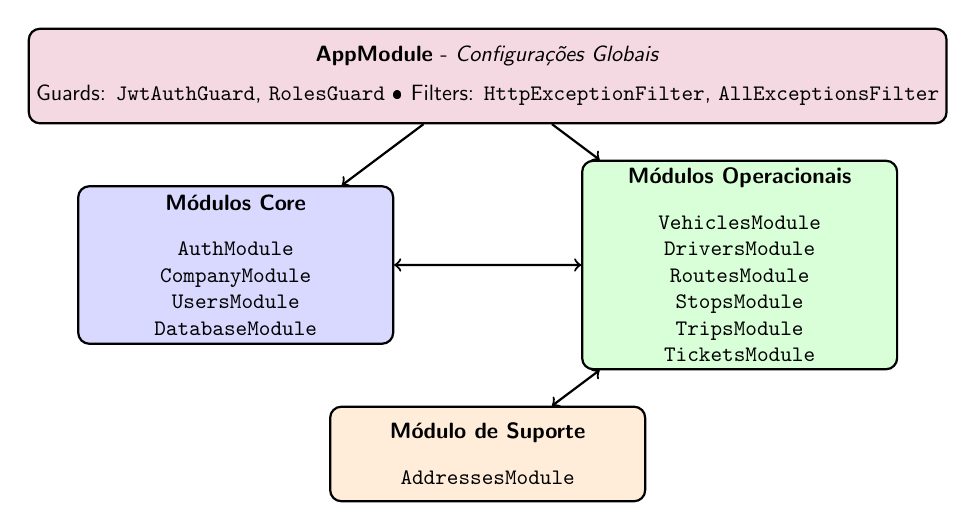
\begin{tikzpicture}[scale=0.8, every node/.style={transform shape}]
  % Módulos Core
  \node[draw, rounded corners, thick, fill=blue!15, minimum width=5cm, minimum height=2.5cm, align=center] (core) at (0,3) {
    \textbf{Módulos Core}\\[0.3cm]
    \texttt{AuthModule}\\
    \texttt{CompanyModule}\\
    \texttt{UsersModule}\\
    \texttt{DatabaseModule}
  };
  
  % Módulos Operacionais
  \node[draw, rounded corners, thick, fill=green!15, minimum width=5cm, minimum height=3cm, align=center] (operational) at (8,3) {
    \textbf{Módulos Operacionais}\\[0.3cm]
    \texttt{VehiclesModule}\\
    \texttt{DriversModule}\\
    \texttt{RoutesModule}\\
    \texttt{StopsModule}\\
    \texttt{TripsModule}\\
    \texttt{TicketsModule}
  };
  
  % Módulos de Suporte
  \node[draw, rounded corners, thick, fill=orange!15, minimum width=5cm, minimum height=1.5cm, align=center] (support) at (4,0) {
    \textbf{Módulo de Suporte}\\[0.3cm]
    \texttt{AddressesModule}
  };
  
  % AppModule
  \node[draw, rounded corners, thick, fill=purple!15, minimum width=10cm, minimum height=1.5cm, align=center] (app) at (4,6) {
    \textbf{AppModule} - \textit{Configurações Globais}\\[0.2cm]
    Guards: \texttt{JwtAuthGuard}, \texttt{RolesGuard} • Filters: \texttt{HttpExceptionFilter}, \texttt{AllExceptionsFilter}
  };
  
  % Setas
  \draw[->, thick] (app) -- (core);
  \draw[->, thick] (app) -- (operational);
  \draw[<->, thick] (core) -- (operational);
  \draw[<->, thick] (support) -- (operational);
\end{tikzpicture}
\caption{Organização modular do backend BusLy.}
\label{fig:backend-modules}
\end{figure}

\subsection{Pipeline de Processamento}

Cada requisição HTTP passa por um pipeline estruturado de middleware, guards, interceptors e filters, garantindo segurança e consistência.

\begin{figure}[H]
\centering
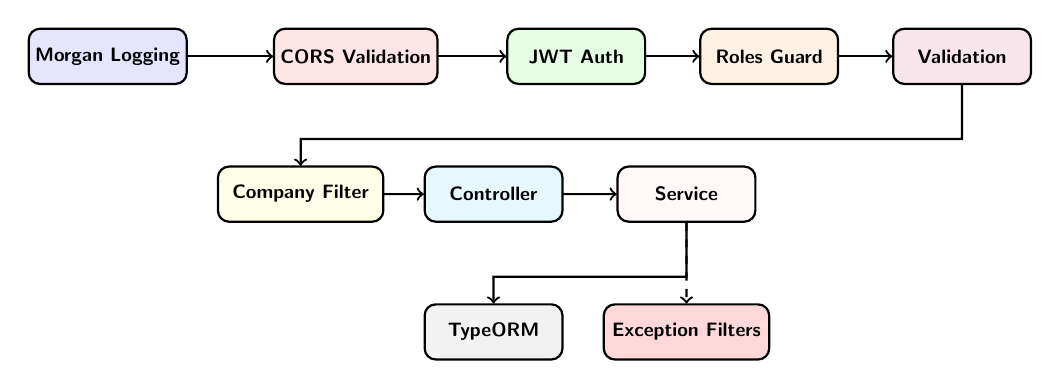
\begin{tikzpicture}[scale=0.7, every node/.style={transform shape}]
  % Pipeline stages
  \node[draw, rounded corners, thick, fill=blue!10, minimum width=2.5cm, minimum height=1cm] (morgan) at (0,0) {\textbf{Morgan Logging}};
  \node[draw, rounded corners, thick, fill=red!10, minimum width=2.5cm, minimum height=1cm] (cors) at (4.5,0) {\textbf{CORS Validation}};
  \node[draw, rounded corners, thick, fill=green!10, minimum width=2.5cm, minimum height=1cm] (jwt) at (8.5,0) {\textbf{JWT Auth}};
  \node[draw, rounded corners, thick, fill=orange!10, minimum width=2.5cm, minimum height=1cm] (roles) at (12,0) {\textbf{Roles Guard}};
  \node[draw, rounded corners, thick, fill=purple!10, minimum width=2.5cm, minimum height=1cm] (validation) at (15.5,0) {\textbf{Validation}};
  
  \node[draw, rounded corners, thick, fill=yellow!10, minimum width=3cm, minimum height=1cm] (interceptor) at (3.5,-2.5) {\textbf{Company Filter}};
  \node[draw, rounded corners, thick, fill=cyan!10, minimum width=2.5cm, minimum height=1cm] (controller) at (7,-2.5) {\textbf{Controller}};
  \node[draw, rounded corners, thick, fill=pink!10, minimum width=2.5cm, minimum height=1cm] (service) at (10.5,-2.5) {\textbf{Service}};
  
  \node[draw, rounded corners, thick, fill=gray!10, minimum width=2.5cm, minimum height=1cm] (typeorm) at (7,-5) {\textbf{TypeORM}};
  \node[draw, rounded corners, thick, fill=red!15, minimum width=3cm, minimum height=1cm] (filters) at (10.5,-5) {\textbf{Exception Filters}};
  
  % Arrows
  \draw[->, thick] (morgan) -- (cors);
  \draw[->, thick] (cors) -- (jwt);
  \draw[->, thick] (jwt) -- (roles);
  \draw[->, thick] (roles) -- (validation);
  \draw[->, thick] (validation) -- ++(0,-1.5) -| (interceptor);
  \draw[->, thick] (interceptor) -- (controller);
  \draw[->, thick] (controller) -- (service);
  \draw[->, thick] (service) -- ++(0,-1.5) -| (typeorm);
  \draw[->, thick, dashed] (service) -- (filters);
\end{tikzpicture}
\caption{Pipeline de processamento de requisições.}
\label{fig:request-pipeline}
\end{figure}

\subsection{Fluxo de Autenticação}

O sistema utiliza autenticação baseada em JWT com suporte a multi-tenancy. A Figura~\ref{fig:auth-sequence} detalha o processo completo.

\begin{figure}[H]
\centering
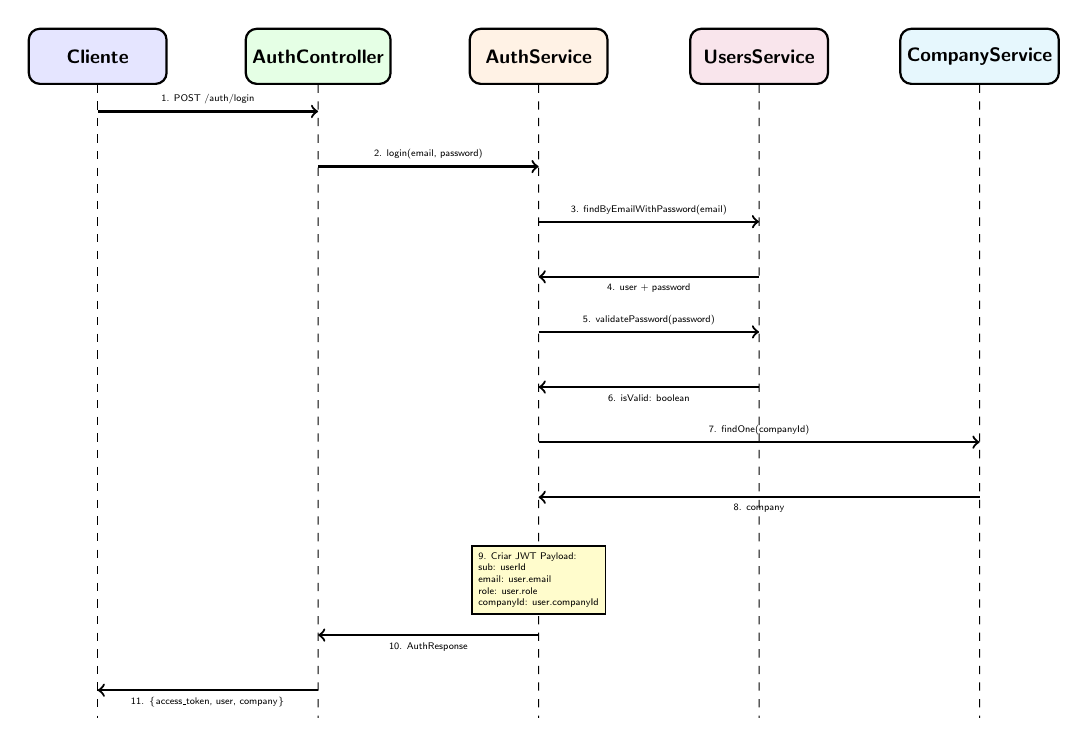
\begin{tikzpicture}[scale=0.7, every node/.style={transform shape}]
  % Participantes
  \node[draw, rounded corners, thick, fill=blue!10, minimum width=2.5cm, minimum height=1cm] (client) at (0,11) {\textbf{Cliente}};
  \node[draw, rounded corners, thick, fill=green!10, minimum width=2.5cm, minimum height=1cm] (auth) at (4,11) {\textbf{AuthController}};
  \node[draw, rounded corners, thick, fill=orange!10, minimum width=2.5cm, minimum height=1cm] (service) at (8,11) {\textbf{AuthService}};
  \node[draw, rounded corners, thick, fill=purple!10, minimum width=2.5cm, minimum height=1cm] (users) at (12,11) {\textbf{UsersService}};
  \node[draw, rounded corners, thick, fill=cyan!10, minimum width=2.5cm, minimum height=1cm] (company) at (16,11) {\textbf{CompanyService}};
  
  % Linhas de vida
  \draw[dashed] (client) -- (0,-1);
  \draw[dashed] (auth) -- (4,-1);
  \draw[dashed] (service) -- (8,-1);
  \draw[dashed] (users) -- (12,-1);
  \draw[dashed] (company) -- (16,-1);
  
  % Mensagens
  \draw[->, thick] (0,10) -- node[above, font=\tiny]{1. POST /auth/login} (4,10);
  \draw[->, thick] (4,9) -- node[above, font=\tiny]{2. login(email, password)} (8,9);
  \draw[->, thick] (8,8) -- node[above, font=\tiny]{3. findByEmailWithPassword(email)} (12,8);
  \draw[<-, thick] (8,7) -- node[below, font=\tiny]{4. user + password} (12,7);
  \draw[->, thick] (8,6) -- node[above, font=\tiny]{5. validatePassword(password)} (12,6);
  \draw[<-, thick] (8,5) -- node[below, font=\tiny]{6. isValid: boolean} (12,5);
  \draw[->, thick] (8,4) -- node[above, font=\tiny]{7. findOne(companyId)} (16,4);
  \draw[<-, thick] (8,3) -- node[below, font=\tiny]{8. company} (16,3);
  
  % Processamento interno
  \node[draw, fill=yellow!20, align=left, font=\tiny] at (8,1.5) {9. Criar JWT Payload:\\sub: userId\\email: user.email\\role: user.role\\companyId: user.companyId};
  
  \draw[<-, thick] (4,0.5) -- node[below, font=\tiny]{10. AuthResponse} (8,0.5);
  \draw[<-, thick] (0,-0.5) -- node[below, font=\tiny]{11. \{access\_token, user, company\}} (4,-0.5);
\end{tikzpicture}
\caption{Diagrama de sequência - fluxo de autenticação.}
\label{fig:auth-sequence}
\end{figure}

\subsection{Arquitetura Multi-tenant}

O sistema implementa isolamento de dados por empresa através do padrão \texttt{BaseCompanyService}, que injeta automaticamente o \texttt{companyId} em todas as operações de banco de dados. O \texttt{CompanyFilterInterceptor} extrai o contexto da empresa do token JWT e disponibiliza para os serviços.

\begin{itemize}
  \item \textbf{Isolamento Automático}: Todas as entidades operacionais possuem \texttt{companyId}
  \item \textbf{Herança de Comportamento}: Services estendem \texttt{BaseCompanyService<T>}
  \item \textbf{Contexto de Requisição}: Interceptor injeta \texttt{companyId} baseado no token JWT
  \item \textbf{Validação de Acesso}: Queries automáticas com filtro por empresa
\end{itemize}

\section{Arquitetura do Frontend}
O frontend emprega Next.js~15 (React~19) com App Router, compondo páginas e layouts por segmentos de negócio (\texttt{/dashboard/[company]/...}). Destacam-se:

\begin{itemize}
  \item \textbf{Sessão e Contexto}: NextAuth com \textit{credentials provider}; o token JWT é persistido na sessão e exposto a componentes via \texttt{useSession} e por um contexto de autenticação.
  \item \textbf{Serviços de API}: um cliente consolidado (\texttt{api.service.ts}) monta a URL base (\texttt{NEXT\_PUBLIC\_API\_URL}), anexa o token \texttt{Bearer}, trata erros e respostas padronizadas e redireciona para login em caso de 401.
  \item \textbf{Camada de UI}: biblioteca de componentes com Radix UI e Tailwind CSS, compondo tabelas, diálogos e formulários tipados com React Hook Form e Zod.
  \item \textbf{Mapas e Geografia}: Leaflet/React-Leaflet para visualização e edição de rotas e paradas (componentes de mapa, formulários e tabelas integrados).
  \item \textbf{Organização por Domínio}: páginas e componentes agrupados por recursos (empresas, motoristas, veículos, rotas, viagens, bilhetes) favorecem coesão e evolução incremental.
\end{itemize}

Essa arquitetura promove: (i) separação de preocupações, (ii) segurança com \textit{JWT} e papéis, (iii) multiempresa por chave de escopo e (iv) escalabilidade via modularização e tipagem estática de ponta a ponta.

% ----------------------------------------------------------
% Modelagem do Projeto
% ----------------------------------------------------------
\chapter{Modelagem do Projeto}

Esta seção deve detalhar como o projeto foi planejado e modelado, incluindo a estrutura e os processos que serão implementados.

As notas de rodapé são detalhadas pela NBR 14724:2011 na seção 5.2.1\footnote{As
notas devem ser digitadas ou datilografadas dentro das margens, ficando
separadas do texto por um espaço simples de entre as linhas e por filete de 5
cm, a partir da margem esquerda. Devem ser alinhadas, a partir da segunda linha
da mesma nota, abaixo da primeira letra da primeira palavra, de forma a destacar
o expoente, sem espaço entre elas e com fonte menor.}

\section{Levantamento de Requisitos}
Descreva o processo de coleta e análise dos requisitos do sistema. Explique como foram identificadas as necessidades dos usuários e as funcionalidades que o software deve oferecer. Inclua requisitos funcionais (o que o sistema deve fazer) e não funcionais (restrições e critérios de qualidade).



\section{ Diagramas de Casos de Uso (opcional)}
Se aplicável, apresente diagramas de casos de uso para ilustrar as interações entre os usuários e o sistema. Explique cada caso de uso e como ele contribui para o funcionamento geral do software.


  \section{Diagramas de Classe (opcional)}
Caso utilizado, descreva os diagramas de classe que representam a estrutura do sistema, incluindo as classes, seus atributos, métodos e relacionamentos. Explique como essas classes se organizam para atender aos requisitos do projeto.

\section{Arquitetura do Sistema}
Descreva a arquitetura geral do sistema, incluindo os componentes principais, suas interações e o fluxo de dados. Pode ser útil incluir diagramas de arquitetura, como MVC (Model-View-Controller) ou microsserviços.

\section{Diagrama de Entidades-Relacionamentos (opcional)}
Se o projeto envolve um banco de dados, apresente o diagrama de entidades-relacionamentos (DER) que modela as tabelas, seus atributos e os relacionamentos entre elas. Explique como o banco de dados foi projetado para atender às necessidades do sistema.

\section{Interface}

Descreva o design da interface do usuário (UI), incluindo aspectos como usabilidade, acessibilidade e experiência do usuário (UX). Se possível, inclua protótipos ou mockups das telas e explique como a interface foi planejada para ser intuitiva e eficiente.

Exemplo de tabela:

\index{tabelas}A \autoref{tab-nivinv} é um exemplo de tabela construída em
\LaTeX.

\begin{table}[htb]
\ABNTEXfontereduzida
\caption[Níveis de investigação]{Níveis de investigação.}
\label{tab-nivinv}
\begin{tabular}{p{2.6cm}|p{6.0cm}|p{2.25cm}|p{3.40cm}}
  %\hline
   \textbf{Nível de Investigação} & \textbf{Insumos}  & \textbf{Sistemas de Investigação}  & \textbf{Produtos}  \\
    \hline
    Meta-nível & Filosofia\index{filosofia} da Ciência  & Epistemologia &
    Paradigma  \\
    \hline
    Nível do objeto & Paradigmas do metanível e evidências do nível inferior &
    Ciência  & Teorias e modelos \\
    \hline
    Nível inferior & Modelos e métodos do nível do objeto e problemas do nível inferior & Prática & Solução de problemas  \\
   % \hline
\end{tabular}
\legend{Fonte: \textcite{van86}}
\end{table}

Já a \autoref{tabela-ibge} apresenta uma tabela criada conforme o padrão do
\textcite{macedo2005} requerido pelas normas da ABNT para documentos técnicos e
acadêmicos.

\begin{table}[htb]
\IBGEtab{%
  \caption{Um Exemplo de tabela alinhada que pode ser longa
  ou curta, conforme padrão IBGE.}%
  \label{tabela-ibge}
}{%
  \begin{tabular}{ccc}
  \toprule
   Nome & Nascimento & Documento \\
  \midrule \midrule
   Maria da Silva & 11/11/1111 & 111.111.111-11 \\
  \midrule 
   João Souza & 11/11/2111 & 211.111.111-11 \\
  \midrule 
   Laura Vicuña & 05/04/1891 & 3111.111.111-11 \\
  \bottomrule
\end{tabular}%
}{%
  \fonte{Produzido pelos autores.}%
  \nota{Esta é uma nota, que diz que os dados são baseados na
  regressão linear.}%
  \nota[Anotações]{Uma anotação adicional, que pode ser seguida de várias
  outras.}%
  }
  \end{table}



\chapter{Software}

Esta seção deve abordar a implementação prática do software, incluindo sua implantação e testes.

\section{Implantação}
Descreva o processo de implantação do software, incluindo os ambientes de desenvolvimento, teste e produção. Explique como o sistema foi configurado e disponibilizado para os usuários finais, incluindo detalhes sobre servidores, containers ou cloud computing, se aplicável.

\section{Testes}
Descreva os tipos de testes realizados (por exemplo, testes unitários, de integração, de carga ou de aceitação) e como eles foram planejados e executados. Explique os critérios de aceitação e os resultados obtidos, destacando eventuais problemas encontrados e como foram resolvidos.


\chapter{Considerações Finais}
\label{cha:consideracoes_finais}

Este trabalho de conclusão de curso abordou o desafio da gestão operacional no setor de transporte rodoviário alternativo de passageiros, um segmento caracterizado pela carência de soluções tecnológicas acessíveis. O problema central identificado foi a dependência de métodos manuais e fragmentados, que resultam em ineficiências e risco de erros. Diante deste cenário, o objetivo geral do projeto foi desenvolver um protótipo funcional de uma plataforma web, no modelo \textit{Software as a Service} (SaaS), denominada ViaBus, para centralizar e digitalizar essa gestão.

\section{Conclusão}

Conclui-se que o objetivo geral do trabalho foi atingido, uma vez que o protótipo funcional foi desenvolvido e sua arquitetura, detalhada. A implementação materializou os requisitos essenciais levantados na pesquisa de mercado — como o gerenciamento de recursos e a execução de operações de venda —, demonstrando que a abordagem técnica proposta é uma solução plausível para o problema. As contribuições deste projeto são, portanto, de ordem prática e documental: o próprio protótipo funcional, que serve como prova de conceito, e a documentação de uma proposta de arquitetura para a construção de um sistema SaaS \textit{multi-tenant} focado neste nicho de mercado.

\section{Limitações do Trabalho}

É fundamental reconhecer as limitações inerentes a este trabalho para contextualizar o alcance de suas conclusões. A principal limitação metodológica reside na pesquisa de mercado, conduzida com uma amostra de apenas dois gestores, o que não permite a generalização estatística dos achados. No que tange à validação, a utilização de uma Avaliação Heurística em vez de testes com usuários finais oferece conclusões de usabilidade de caráter preliminar. Por fim, o escopo do protótipo funcional foi deliberadamente focado na perspectiva do gestor, não incluindo o desenvolvimento de uma aplicação para o passageiro e motorista, funcionalidades apontadas como relevantes na pesquisa.

\section{Trabalhos Futuros}

Com base nas limitações apontadas, delineia-se um caminho claro para a evolução do projeto. Recomenda-se, primeiramente, a validação da solução em maior escala, através de uma pesquisa de mercado quantitativa e da condução de testes de usabilidade com usuários reais. Em paralelo, o desenvolvimento do protótipo pode avançar com a implementação de funcionalidades de relatório (RF11) e do manifesto de viagem para o motorista (RF09). A criação de um único e versátil aplicativo móvel que, por meio de perfis de usuário distintos, atenderia tanto ao passageiro — com funcionalidades para a compra de bilhetes e o rastreamento de viagens — quanto ao motorista — oferecendo ferramentas para o controle digital do embarque — e a integração com sistemas de pagamento online representam os passos subsequentes para transformar o protótipo em um produto de mercado.

%% Finalizações para o PDF
\bookmarksetup{startatroot}

%% Elementos pós-textuais: Referências, Anexos, etc.
%% %%%%%%%%%%%%%%%%%%%%%%%%%%%%%%%%%%%%%%%%% %%
%% Elementos Pós Textuais
%% ----------------------
%% 
%% Segundo o manual do IFPI, eles devem ser os seguintes (nessa ordem):
%% 1. Referências (obrigatório)
%% 2. Glossário (opcional)
%% 3. Apêndice (opcional)
%% 4. Anexos (opcional)
%% 5. Índices (opcional)
%% %%%%%%%%%%%%%%%%%%%%%%%%%%%%%%%%%%%%%%%%% %%

%% Indica ao LaTeX que a partir deste ponto ficarão os elementos pós-textuais
\postextual

%% 01: Referências bibliográficas
%% Referências bibliográficas

% \bibliography{bibliografia}
\printbibliography

%% 02: Glossário
%% Glossário
%\glossary

%% 03: Apêndices
%% Apêndices

%\begin{apendicesenv}
%
%%% Imprime uma página indicando o início dos apêndices (opcional, comente para retirar)
%\partapendices
%
%%% Cada Capítulo será um apêndice
%\chapter{Este será o apêndice A}
%Lorem ipsum dolor sit amet, consectetur adipiscing elit. Praesent congue, turpis quis rutrum fringilla, lacus lorem faucibus diam, sit amet viverra urna quam sed metus. Pellentesque quis eros ex. Nullam vel ante rutrum eros placerat egestas. Morbi volutpat sapien elementum tincidunt fringilla. Class aptent taciti sociosqu ad litora torquent per conubia nostra, per inceptos himenaeos. Sed rutrum vestibulum bibendum. Sed tincidunt, magna sit amet tempor tincidunt, turpis neque blandit eros, a tincidunt felis mauris vitae est. Aliquam sit amet placerat risus. Nunc eget est pulvinar est tristique convallis sit amet vel risus. Maecenas turpis nisl, blandit ac porttitor non, ultrices id est. Cras eleifend nulla ut condimentum ullamcorper. Quisque at gravida massa, fringilla varius sapien. Nulla ullamcorper mauris vel ipsum elementum, vel tincidunt ante pretium. Ut iaculis nunc ex, vitae elementum ante efficitur non. Pellentesque venenatis tristique odio, nec volutpat dui dapibus sit amet. Maecenas eu velit at arcu hendrerit sagittis vel a odio.
%
%Nulla gravida metus at gravida ultricies. Nulla auctor id mi id suscipit. Proin vestibulum metus non eros feugiat, ac blandit diam vestibulum. Sed in arcu eget mauris rhoncus semper. Integer dignissim dui quis massa vestibulum, luctus ultrices metus mollis. Sed aliquam leo hendrerit lacus ultricies efficitur. Praesent quis quam sed lorem tincidunt fringilla non interdum odio. Phasellus vel enim mattis, tempor arcu ut, pulvinar est. Sed ut tempus est. Fusce erat nisi, scelerisque quis tellus sit amet, lacinia sagittis libero. Sed ultrices odio ipsum, ut vestibulum nulla auctor in.
%
%
%
%
%
%\chapter{Este será o apêndice B}
%Lorem ipsum dolor sit amet, consectetur adipiscing elit. Integer malesuada elit vel lacus fringilla, in luctus orci finibus. Praesent eget augue et enim luctus cursus ut ac nisl. In lobortis tellus non mauris euismod, tempus hendrerit nisi euismod. Integer id magna sapien. Nunc urna magna, consequat sed vehicula quis, convallis non justo. Aliquam risus dolor, viverra quis dignissim eget, convallis id sapien. Ut id turpis suscipit, mollis quam sed, lacinia lacus. Donec ac nulla dui.
%
%
%\end{apendicesenv}

%% 04: Anexos
%% Anexos
\begin{anexosenv}

%% Imprime uma página indicando o início dos anexos (opcional, comente para retirar)
%\partanexos

% Exemplo de inclusão
% \input{pos-textual/anexo} 
\chapter{TRECHO DA CARTA DE PERO VAZ DE CAMINHA} \label{anexo:a}
\vspace{-2cm}
\begin{figure}[H]
	\caption*{}
	\begin{center}
	    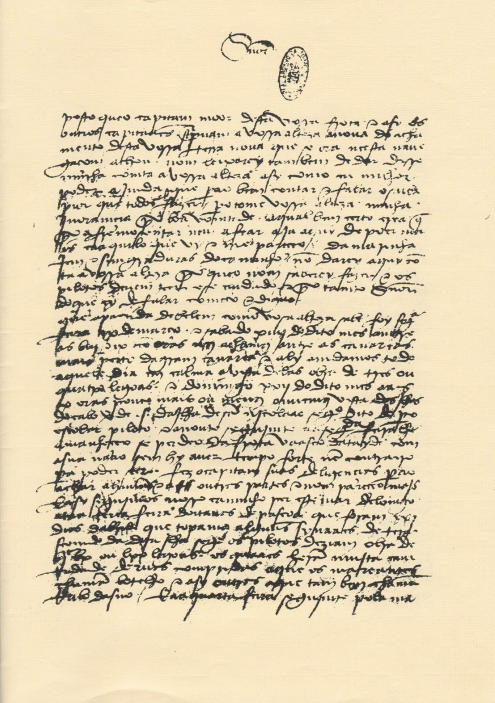
\includegraphics[scale=1.0]{imagens/carta_pero_vaz.png}
	\end{center}
	
\end{figure}


\end{anexosenv}

%% 05: Índices
%% Índices
%\phantompart \printindex

%% Capa do CD (opcional)
%%% Isso aqui cria a capa do CD, no final do documento :)
\newpage
\thispagestyle{empty}
\begin{center}
\covers[{\vspace{1.5cm} \Large \MakeUppercase{Curso de \imprimirnomedocurso} \\ \vspace{1cm} \textbf{\imprimirautor} \\ \vspace{0.5cm} {TÍTULO: \imprimirtitulo}}]{
	{\vspace{1.5cm} 
\includegraphics[scale=0.25]{imagens/IFPI.png} \\ \vspace{1cm} \MakeUppercase{Curso de \imprimirnomedocurso} \\ \vspace{1cm} {\textbf{\imprimirautor}} \\ \vspace{0.3cm} {TÍTULO: \imprimirtitulo} \\ \vspace{1.5cm} \MakeUppercase{\imprimirlocal} \par \imprimirdata}
}{
	\MakeUppercase{\tiny \imprimirtitulo}
}
\end{center}

\end{document}